% =============================================================================
%  Manuscript for the Journal of Computational Science (Elsevier, elsarticle).
%  Supplementary Material in si.tex. Build:
%    pdflatex si && pdflatex jcs && bibtex jcs && pdflatex jcs && pdflatex jcs
%  (si first: S-numbered references are imported through xr). Every number comes from the
%  numeros*.tex files written by the analysis scripts (see ../actualizar.sh).
%  jcim.tex keeps the version submitted to J. Chem. Inf. Model. (desk-rejected 2026-11-03).
% =============================================================================
\documentclass[preprint,12pt]{elsarticle}
\usepackage[T1]{fontenc}
\usepackage{lmodern}
\usepackage{amsmath,amssymb}
\usepackage{booktabs}
\usepackage{array}
\usepackage{graphicx}
\usepackage{siunitx}
\usepackage{xcolor}
\usepackage{enumitem}
\usepackage[section]{placeins}
\usepackage{xr-hyper}
\usepackage{xurl}
\usepackage[hidelinks]{hyperref}
\usepackage[capitalise]{cleveref}
\externaldocument{si}
\biboptions{sort&compress}
% Macros compartidas por jcim.tex (manuscrito) y si.tex (Supporting Information).
% Todas las cifras proceden de los ficheros numeros*.tex generados por los scripts; no se escriben a mano.
% Generado por hacer_numeros.py a partir de resultados/preliminar.json. No editar a mano.
\newcommand{\nShort}{6{,}137}
\newcommand{\nLong}{133}
\newcommand{\nTotal}{6{,}270}
\newcommand{\betaShortMed}{0.43}
\newcommand{\betaShortLo}{0.26}
\newcommand{\betaShortHi}{0.60}
\newcommand{\betaShortSubPct}{97.8}
\newcommand{\betaShortDiffPct}{0.03}
\newcommand{\betaShortDiffN}{2}
\newcommand{\betaLongMed}{0.65}
\newcommand{\betaLongLo}{0.49}
\newcommand{\betaLongHi}{0.83}
\newcommand{\betaLongSubPct}{69.2}
\newcommand{\betaLongDiffPct}{3.8}
\newcommand{\betaLongDiffN}{5}
\newcommand{\epSd}{0.19}
\newcommand{\epFactor}{1.21}
\newcommand{\epOutOnePointFivePct}{5.4}
\newcommand{\epOutTwoPct}{0.2}
\newcommand{\epRho}{0.92}
\newcommand{\ratioHalf}{8.86}
\newcommand{\ratioHalfLo}{4.70}
\newcommand{\ratioHalfHi}{12.47}
\newcommand{\rhoHalf}{0.91}
\newcommand{\withinHalfPct}{0.0}
\newcommand{\ratioOne}{5.23}
\newcommand{\ratioOneLo}{3.12}
\newcommand{\ratioOneHi}{7.26}
\newcommand{\rhoOne}{0.92}
\newcommand{\withinOnePct}{0.0}
\newcommand{\ratioTwo}{3.34}
\newcommand{\ratioTwoLo}{2.15}
\newcommand{\ratioTwoHi}{4.32}
\newcommand{\rhoTwo}{0.94}
\newcommand{\withinTwoPct}{0.0}
\newcommand{\ratioFive}{1.95}
\newcommand{\ratioFiveLo}{1.47}
\newcommand{\ratioFiveHi}{2.40}
\newcommand{\rhoFive}{0.96}
\newcommand{\withinFivePct}{0.8}
\newcommand{\ratioTen}{1.40}
\newcommand{\ratioTenLo}{1.18}
\newcommand{\ratioTenHi}{1.63}
\newcommand{\rhoTen}{0.98}
\newcommand{\withinTenPct}{16.5}
\newcommand{\ratioFifteen}{1.19}
\newcommand{\ratioFifteenLo}{1.08}
\newcommand{\ratioFifteenHi}{1.31}
\newcommand{\rhoFifteen}{0.99}
\newcommand{\withinFifteenPct}{73.7}
\newcommand{\ratioTwenty}{1.07}
\newcommand{\ratioTwentyLo}{1.03}
\newcommand{\ratioTwentyHi}{1.12}
\newcommand{\rhoTwenty}{1.00}
\newcommand{\withinTwentyPct}{100.0}
\newcommand{\nPairs}{133}
\newcommand{\PairEndRatio}{2.90}
\newcommand{\PairEndLo}{1.58}
\newcommand{\PairEndHi}{4.74}
\newcommand{\PairEndRho}{0.84}
\newcommand{\PairEndRecall}{85}
\newcommand{\PairAvgRatio}{3.90}
\newcommand{\PairAvgLo}{2.14}
\newcommand{\PairAvgHi}{6.22}
\newcommand{\PairAvgRho}{0.85}
\newcommand{\PairAvgRecall}{81}
\newcommand{\nLongLit}{37}
\newcommand{\nLongScreen}{96}
\newcommand{\nRep}{94}
\newcommand{\sdLong}{0.98}
\newcommand{\RepEndRho}{0.48}
\newcommand{\RepEndFactor}{1.43}
\newcommand{\RepEndSd}{0.35}
\newcommand{\RepEndDiffPct}{38}
\newcommand{\RepEndIcc}{0.44}
\newcommand{\RepEndSdAll}{0.49}
\newcommand{\RepEndSdSub}{0.44}
\newcommand{\RepAvgRho}{0.56}
\newcommand{\RepAvgFactor}{1.32}
\newcommand{\RepAvgSd}{0.28}
\newcommand{\RepAvgDiffPct}{32}
\newcommand{\RepAvgIcc}{0.54}
\newcommand{\RepAvgSdAll}{0.43}
\newcommand{\RepAvgSdSub}{0.40}
\newcommand{\RepBetaSd}{0.15}
\newcommand{\RepBetaRho}{-0.07}
\newcommand{\nPrefix}{133}
\newcommand{\valMaxDev}{5e-7}
\newcommand{\driftMed}{1.2}
\newcommand{\driftMax}{34}
\newcommand{\driftFracPct}{63}
\newcommand{\preEndRatioTwo}{4.43}
\newcommand{\preEndErrTwo}{4.43}
\newcommand{\preEndCovTwo}{1}
\newcommand{\preEndRhoTwo}{0.79}
\newcommand{\preEndRatioFive}{2.83}
\newcommand{\preEndErrFive}{2.83}
\newcommand{\preEndCovFive}{3}
\newcommand{\preEndRhoFive}{0.81}
\newcommand{\preEndRatioTen}{2.02}
\newcommand{\preEndErrTen}{2.02}
\newcommand{\preEndCovTen}{14}
\newcommand{\preEndRhoTen}{0.84}
\newcommand{\preEndRatioTwenty}{1.43}
\newcommand{\preEndErrTwenty}{1.45}
\newcommand{\preEndCovTwenty}{47}
\newcommand{\preEndRhoTwenty}{0.87}
\newcommand{\preHalfRatioTwo}{6.39}
\newcommand{\preHalfErrTwo}{6.39}
\newcommand{\preHalfCovTwo}{0}
\newcommand{\preHalfRhoTwo}{0.80}
\newcommand{\preHalfRatioFive}{4.05}
\newcommand{\preHalfErrFive}{4.05}
\newcommand{\preHalfCovFive}{0}
\newcommand{\preHalfRhoFive}{0.81}
\newcommand{\preHalfRatioTen}{2.55}
\newcommand{\preHalfErrTen}{2.55}
\newcommand{\preHalfCovTen}{2}
\newcommand{\preHalfRhoTen}{0.83}
\newcommand{\preHalfRatioTwenty}{1.78}
\newcommand{\preHalfErrTwenty}{1.78}
\newcommand{\preHalfCovTwenty}{12}
\newcommand{\preHalfRhoTwenty}{0.89}
\newcommand{\preFitRatioTwo}{2.83}
\newcommand{\preFitErrTwo}{2.85}
\newcommand{\preFitCovTwo}{23}
\newcommand{\preFitRhoTwo}{0.71}
\newcommand{\preFitRatioFive}{2.02}
\newcommand{\preFitErrFive}{2.02}
\newcommand{\preFitCovFive}{39}
\newcommand{\preFitRhoFive}{0.74}
\newcommand{\preFitRatioTen}{1.48}
\newcommand{\preFitErrTen}{1.51}
\newcommand{\preFitCovTen}{56}
\newcommand{\preFitRhoTen}{0.78}
\newcommand{\preFitRatioTwenty}{1.16}
\newcommand{\preFitErrTwenty}{1.24}
\newcommand{\preFitCovTwenty}{78}
\newcommand{\preFitRhoTwenty}{0.85}
\newcommand{\prePowRatioTwo}{0.72}
\newcommand{\prePowErrTwo}{1.50}
\newcommand{\prePowCovTwo}{59}
\newcommand{\prePowRhoTwo}{0.72}
\newcommand{\prePowRatioFive}{0.95}
\newcommand{\prePowErrFive}{1.37}
\newcommand{\prePowCovFive}{68}
\newcommand{\prePowRhoFive}{0.75}
\newcommand{\prePowRatioTen}{1.07}
\newcommand{\prePowErrTen}{1.26}
\newcommand{\prePowCovTen}{74}
\newcommand{\prePowRhoTen}{0.79}
\newcommand{\prePowRatioTwenty}{1.11}
\newcommand{\prePowErrTwenty}{1.20}
\newcommand{\prePowCovTwenty}{74}
\newcommand{\prePowRhoTwenty}{0.87}
\newcommand{\ruleBetaNineStopPct}{3}
\newcommand{\ruleBetaNineTime}{49.3}
\newcommand{\ruleBetaNineErr}{1.37}
\newcommand{\ruleBetaNineErrStop}{1.38}
\newcommand{\ruleBetaNineTimeStop}{26.8}
\newcommand{\ruleBetaEightStopPct}{19}
\newcommand{\ruleBetaEightTime}{44.6}
\newcommand{\ruleBetaEightErr}{1.39}
\newcommand{\ruleBetaEightErrStop}{1.39}
\newcommand{\ruleBetaEightTimeStop}{21.2}
\newcommand{\ruleCvTenStopPct}{2}
\newcommand{\ruleCvTenTime}{49.3}
\newcommand{\ruleCvTenErr}{1.37}
\newcommand{\ruleCvTenErrStop}{1.36}
\newcommand{\ruleCvTenTimeStop}{21.0}
\newcommand{\ruleCvTwentyStopPct}{80}
\newcommand{\ruleCvTwentyTime}{15.6}
\newcommand{\ruleCvTwentyErr}{1.79}
\newcommand{\ruleCvTwentyErrStop}{2.22}
\newcommand{\ruleCvTwentyTimeStop}{7.3}
\newcommand{\ruleCvPowStopPct}{24}
\newcommand{\ruleCvPowTime}{43.4}
\newcommand{\ruleCvPowErr}{1.04}
\newcommand{\ruleCvPowErrStop}{1.13}
\newcommand{\ruleCvPowTimeStop}{22.7}
\newcommand{\ScrTopFiveK}{5}
\newcommand{\ScrTopFiveHits}{4}
\newcommand{\ScrTopFiveRecall}{80}
\newcommand{\LitInTopFive}{7}
\newcommand{\ScrTopTenK}{10}
\newcommand{\ScrTopTenHits}{7}
\newcommand{\ScrTopTenRecall}{70}
\newcommand{\LitInTopTen}{13}
\newcommand{\ScrTopTwentyK}{19}
\newcommand{\ScrTopTwentyHits}{14}
\newcommand{\ScrTopTwentyRecall}{74}
\newcommand{\LitInTopTwenty}{24}
\newcommand{\ScrN}{96}
\newcommand{\sensLongSubMinPct}{46}
\newcommand{\sensLongSubMaxPct}{81}
\newcommand{\sensLongDiffMinN}{0}
\newcommand{\sensLongDiffMaxN}{19}
\newcommand{\RepEndIccLo}{0.27}
\newcommand{\RepEndIccHi}{0.61}
\newcommand{\RepEndIccSub}{0.53}
\newcommand{\RepEndIccSubLo}{0.34}
\newcommand{\RepEndIccSubHi}{0.66}
\newcommand{\RepEndPairFactor}{1.65}
\newcommand{\RepEndPairFactorNinetyFive}{2.67}
\newcommand{\RepAvgIccLo}{0.40}
\newcommand{\RepAvgIccHi}{0.67}
\newcommand{\RepAvgIccSub}{0.62}
\newcommand{\RepAvgIccSubLo}{0.45}
\newcommand{\RepAvgIccSubHi}{0.74}
\newcommand{\RepAvgPairFactor}{1.48}
\newcommand{\RepAvgPairFactorNinetyFive}{2.16}
\newcommand{\PairEndRhoLo}{0.76}
\newcommand{\PairEndRhoHi}{0.89}
\newcommand{\PairEndRhoScreen}{0.68}
\newcommand{\PairEndRhoLit}{0.93}
\newcommand{\PairEndTopFiveK}{7}
\newcommand{\PairEndTopFiveHits}{7}
\newcommand{\PairEndTopTenK}{13}
\newcommand{\PairEndTopTenHits}{11}
\newcommand{\PairEndTopTwentyK}{27}
\newcommand{\PairEndTopTwentyHits}{23}
\newcommand{\PairAvgRhoLo}{0.76}
\newcommand{\PairAvgRhoHi}{0.90}
\newcommand{\PairAvgRhoScreen}{0.70}
\newcommand{\PairAvgRhoLit}{0.94}
\newcommand{\PairAvgTopFiveK}{7}
\newcommand{\PairAvgTopFiveHits}{6}
\newcommand{\PairAvgTopTenK}{13}
\newcommand{\PairAvgTopTenHits}{10}
\newcommand{\PairAvgTopTwentyK}{27}
\newcommand{\PairAvgTopTwentyHits}{22}
\newcommand{\tamNAtomsMed}{6{,}002}
\newcommand{\tamNAtomsMin}{2{,}328}
\newcommand{\tamNAtomsMax}{7{,}541}
\newcommand{\tamChainsMed}{9}
\newcommand{\tamChainsMin}{1}
\newcommand{\tamChainsMax}{15}
\newcommand{\tamBoxMin}{3.0}
\newcommand{\tamBoxMax}{4.2}
\newcommand{\tamBoxMed}{4.0}
\newcommand{\tamNIons}{50}
\newcommand{\tamIonsAllEqual}{1}
\newcommand{\tamNRecount}{125}
\newcommand{\nOnlyReplica}{1}
\newcommand{\techoEndOneStructMax}{0.58}
\newcommand{\mlLeakPairs}{77}
\newcommand{\mlLeakSameFold}{17}
\newcommand{\mlCeilRatio}{1.05}
\newcommand{\mlCeilRatioLo}{0.89}
\newcommand{\mlCeilRatioHi}{1.35}
\newcommand{\alRoundsTopOne}{6}
\newcommand{\alRoundsTopTen}{18}
\newcommand{\alBatchPct}{5}
\newcommand{\alSdSys}{0.31}
\newcommand{\alNoiseA}{0.35}
\newcommand{\alNoiseB}{-0.067}

% Generado por referencias.py a partir de resultados/referencias.json. No editar a mano.
\newcommand{\refN}{133}
\newcommand{\refSlopeVsDapp}{0.70}
\newcommand{\refPowErrMin}{1.33}
\newcommand{\refPowErrMax}{1.45}
\newcommand{\refPowBiasMin}{0.83}
\newcommand{\refPowBiasMax}{1.06}
\newcommand{\refEndErrMin}{2.37}
\newcommand{\refEndErrMax}{3.27}
\newcommand{\refEndBiasMin}{2.37}
\newcommand{\refEndBiasMax}{3.27}
\newcommand{\refFitErrMin}{1.80}
\newcommand{\refFitErrMax}{2.33}
\newcommand{\refFitBiasMin}{1.73}
\newcommand{\refFitBiasMax}{2.33}
\newcommand{\refPowSlopeErrFive}{1.99}
\newcommand{\refPowSlopeRatioFive}{0.54}
\newcommand{\refBracketFivePct}{78}
\newcommand{\refPowSlopeErrTen}{1.52}
\newcommand{\refPowSlopeRatioTen}{0.68}
\newcommand{\refBracketTenPct}{73}
\newcommand{\refPowSlopeErrTwenty}{1.36}
\newcommand{\refPowSlopeRatioTwenty}{0.77}
\newcommand{\refBracketTwentyPct}{69}
\newcommand{\refEndSlopeErrFive}{4.01}
\newcommand{\refFitSlopeErrFive}{3.05}

% Generado por frontera.py a partir de resultados/frontera.json. No editar a mano.
\newcommand{\frN}{133}
\newcommand{\frSplits}{500}
\newcommand{\frMinFixEndOneFive}{20.0}
\newcommand{\frTestFixEndOneFive}{20.0}
\newcommand{\frMetFixEndOneFive}{97}
\newcommand{\frMinFixFitOneFive}{12.0}
\newcommand{\frTestFixFitOneFive}{12.0}
\newcommand{\frMetFixFitOneFive}{61}
\newcommand{\frMinFixPowOneFive}{2.0}
\newcommand{\frTestFixPowOneFive}{2.0}
\newcommand{\frMetFixPowOneFive}{59}
\newcommand{\frMinRegimeOneFive}{34.7}
\newcommand{\frTestRegimeOneFive}{35.2}
\newcommand{\frMetRegimeOneFive}{64}
\newcommand{\frMinPrecFitOneFive}{36.2}
\newcommand{\frTestPrecFitOneFive}{37.0}
\newcommand{\frMetPrecFitOneFive}{67}
\newcommand{\frMinPrecPowOneFive}{11.5}
\newcommand{\frTestPrecPowOneFive}{11.9}
\newcommand{\frMetPrecPowOneFive}{76}
\newcommand{\frMinFixEndOneThree}{30.0}
\newcommand{\frTestFixEndOneThree}{30.0}
\newcommand{\frMetFixEndOneThree}{84}
\newcommand{\frMinFixFitOneThree}{20.0}
\newcommand{\frTestFixFitOneThree}{20.0}
\newcommand{\frMetFixFitOneThree}{96}
\newcommand{\frMinFixPowOneThree}{10.0}
\newcommand{\frTestFixPowOneThree}{7.5}
\newcommand{\frMetFixPowOneThree}{45}
\newcommand{\frMinRegimeOneThree}{n/a}
\newcommand{\frTestRegimeOneThree}{n/a}
\newcommand{\frMetRegimeOneThree}{0}
\newcommand{\frMinPrecFitOneThree}{n/a}
\newcommand{\frTestPrecFitOneThree}{50.0}
\newcommand{\frMetPrecFitOneThree}{0}
\newcommand{\frMinPrecPowOneThree}{21.0}
\newcommand{\frTestPrecPowOneThree}{20.9}
\newcommand{\frMetPrecPowOneThree}{93}
\newcommand{\frMinFixEndOneTwo}{40.0}
\newcommand{\frTestFixEndOneTwo}{40.0}
\newcommand{\frMetFixEndOneTwo}{79}
\newcommand{\frMinFixFitOneTwo}{n/a}
\newcommand{\frTestFixFitOneTwo}{25.0}
\newcommand{\frMetFixFitOneTwo}{0}
\newcommand{\frMinFixPowOneTwo}{20.0}
\newcommand{\frTestFixPowOneTwo}{20.0}
\newcommand{\frMetFixPowOneTwo}{50}
\newcommand{\frMinRegimeOneTwo}{n/a}
\newcommand{\frTestRegimeOneTwo}{n/a}
\newcommand{\frMetRegimeOneTwo}{0}
\newcommand{\frMinPrecFitOneTwo}{n/a}
\newcommand{\frTestPrecFitOneTwo}{n/a}
\newcommand{\frMetPrecFitOneTwo}{0}
\newcommand{\frMinPrecPowOneTwo}{21.0}
\newcommand{\frTestPrecPowOneTwo}{21.1}
\newcommand{\frMetPrecPowOneTwo}{71}

% Generado por techo.py a partir de resultados/techo.json. No editar a mano.
\newcommand{\techoNRep}{94}
\newcommand{\techoNPairsScreen}{96}
\newcommand{\techoEndCorr}{0.66}
\newcommand{\techoEndCorrLo}{0.52}
\newcommand{\techoEndCorrHi}{0.78}
\newcommand{\techoEndRTwo}{0.44}
\newcommand{\techoEndRelTwo}{0.61}
\newcommand{\techoEndRelFour}{0.76}
\newcommand{\techoEndRepForEight}{6}
\newcommand{\techoEndSdDyn}{0.24}
\newcommand{\techoEndSdStruct}{0.26}
\newcommand{\techoEndFracStructPct}{55}
\newcommand{\techoEndFracStructLo}{28}
\newcommand{\techoEndFracStructHi}{73}
\newcommand{\techoEndShortPrefRatio}{1.00}
\newcommand{\techoEndHetRho}{-0.26}
\newcommand{\techoEndHetP}{0.01}
\newcommand{\techoEndSdSlow}{0.40}
\newcommand{\techoEndSdFast}{0.30}
\newcommand{\techoEndRecallOneTopFive}{36}
\newcommand{\techoEndRecallOneTopTen}{43}
\newcommand{\techoEndRecallOneTopTwenty}{54}
\newcommand{\techoEndRecallTwoTopFive}{46}
\newcommand{\techoEndRecallTwoTopTen}{54}
\newcommand{\techoEndRecallTwoTopTwenty}{63}
\newcommand{\techoEndRecallFourTopFive}{58}
\newcommand{\techoEndRecallFourTopTen}{65}
\newcommand{\techoEndRecallFourTopTwenty}{72}
\newcommand{\techoEndRecallOneTopTenLo}{33}
\newcommand{\techoEndRecallOneTopTenHi}{54}
\newcommand{\techoEndDynN}{96}
\newcommand{\techoEndJointN}{92}
\newcommand{\techoEndJointDiffCorr}{0.53}
\newcommand{\techoEndJointFracStructPct}{57}
\newcommand{\techoEndJointFracStructLo}{44}
\newcommand{\techoEndJointFracStructHi}{69}
\newcommand{\techoEndBatchRepRatio}{1.05}
\newcommand{\techoEndBatchRepP}{0.31}
\newcommand{\techoEndBatchRepRatioLo}{0.95}
\newcommand{\techoEndBatchRepRatioHi}{1.17}
\newcommand{\techoEndBatchPrefRatio}{1.00}
\newcommand{\techoEndBatchPrefP}{0.89}
\newcommand{\techoEndBatchPrefRatioLo}{0.93}
\newcommand{\techoEndBatchPrefRatioHi}{1.06}
\newcommand{\techoEndBatchSdOrig}{0.50}
\newcommand{\techoEndBatchSdRep}{0.53}
\newcommand{\techoEndBatchSdOther}{0.47}
\newcommand{\techoEndBatchLeveneP}{0.67}
\newcommand{\techoEndRelUncentred}{0.44}
\newcommand{\techoEndReprKsRep}{0.61}
\newcommand{\techoEndReprKsLong}{0.65}
\newcommand{\techoEndReprLevRep}{0.82}
\newcommand{\techoEndReprLevLong}{0.65}
\newcommand{\techoEndReprOverlap}{92}
\newcommand{\techoAvgCorr}{0.74}
\newcommand{\techoAvgCorrLo}{0.64}
\newcommand{\techoAvgCorrHi}{0.82}
\newcommand{\techoAvgRTwo}{0.54}
\newcommand{\techoAvgRelTwo}{0.70}
\newcommand{\techoAvgRelFour}{0.83}
\newcommand{\techoAvgRepForEight}{4}
\newcommand{\techoAvgSdDyn}{0.20}
\newcommand{\techoAvgSdStruct}{0.20}
\newcommand{\techoAvgFracStructPct}{51}
\newcommand{\techoAvgFracStructLo}{21}
\newcommand{\techoAvgFracStructHi}{69}
\newcommand{\techoAvgShortPrefRatio}{0.96}
\newcommand{\techoAvgHetRho}{-0.23}
\newcommand{\techoAvgHetP}{0.02}
\newcommand{\techoAvgSdSlow}{0.29}
\newcommand{\techoAvgSdFast}{0.26}
\newcommand{\techoAvgRecallOneTopFive}{43}
\newcommand{\techoAvgRecallOneTopTen}{50}
\newcommand{\techoAvgRecallOneTopTwenty}{59}
\newcommand{\techoAvgRecallTwoTopFive}{53}
\newcommand{\techoAvgRecallTwoTopTen}{61}
\newcommand{\techoAvgRecallTwoTopTwenty}{68}
\newcommand{\techoAvgRecallFourTopFive}{65}
\newcommand{\techoAvgRecallFourTopTen}{70}
\newcommand{\techoAvgRecallFourTopTwenty}{76}
\newcommand{\techoAvgRecallOneTopTenLo}{42}
\newcommand{\techoAvgRecallOneTopTenHi}{58}
\newcommand{\techoAvgDynN}{96}
\newcommand{\techoAvgJointN}{92}
\newcommand{\techoAvgJointDiffCorr}{0.51}
\newcommand{\techoAvgJointFracStructPct}{52}
\newcommand{\techoAvgJointFracStructLo}{33}
\newcommand{\techoAvgJointFracStructHi}{66}
\newcommand{\techoAvgBatchRepRatio}{1.04}
\newcommand{\techoAvgBatchRepP}{0.34}
\newcommand{\techoAvgBatchRepRatioLo}{0.96}
\newcommand{\techoAvgBatchRepRatioHi}{1.12}
\newcommand{\techoAvgBatchPrefRatio}{0.95}
\newcommand{\techoAvgBatchPrefP}{0.10}
\newcommand{\techoAvgBatchPrefRatioLo}{0.91}
\newcommand{\techoAvgBatchPrefRatioHi}{1.01}
\newcommand{\techoAvgBatchSdOrig}{0.45}
\newcommand{\techoAvgBatchSdRep}{0.46}
\newcommand{\techoAvgBatchSdOther}{0.41}
\newcommand{\techoAvgBatchLeveneP}{0.82}
\newcommand{\techoAvgRelUncentred}{0.54}
\newcommand{\techoAvgReprKsRep}{0.78}
\newcommand{\techoAvgReprKsLong}{0.80}
\newcommand{\techoAvgReprLevRep}{0.59}
\newcommand{\techoAvgReprLevLong}{0.48}
\newcommand{\techoAvgReprOverlap}{92}

% Generado por asignacion.py a partir de resultados/asignacion.json. No editar a mano.
\newcommand{\alN}{6{,}003}
\newcommand{\alReps}{200}
\newcommand{\alKurt}{0.13}
\newcommand{\alShapiroP}{0.81}
\newcommand{\alUnifTopOneBOne}{27}
\newcommand{\alUnifTopOneBTwo}{48}
\newcommand{\alHalvingTopOneBTwo}{83}
\newcommand{\alBoundTopOneBTwo}{79}
\newcommand{\alUnifTopOneBFour}{65}
\newcommand{\alHalvingTopOneBFour}{89}
\newcommand{\alBoundTopOneBFour}{86}
\newcommand{\alEqTopOneUnifTwo}{1.1}
\newcommand{\alSavingTopOneUnifTwo}{1.7}
\newcommand{\alEqTopOneUnifThree}{1.2}
\newcommand{\alSavingTopOneUnifThree}{2.5}
\newcommand{\alEqTopOneUnifFour}{1.3}
\newcommand{\alSavingTopOneUnifFour}{3.1}
\newcommand{\alUnifTopFiveBOne}{38}
\newcommand{\alUnifTopFiveBTwo}{55}
\newcommand{\alHalvingTopFiveBTwo}{75}
\newcommand{\alBoundTopFiveBTwo}{74}
\newcommand{\alUnifTopFiveBFour}{68}
\newcommand{\alHalvingTopFiveBFour}{84}
\newcommand{\alBoundTopFiveBFour}{84}
\newcommand{\alEqTopFiveUnifTwo}{1.2}
\newcommand{\alSavingTopFiveUnifTwo}{1.7}
\newcommand{\alEqTopFiveUnifThree}{1.4}
\newcommand{\alSavingTopFiveUnifThree}{2.2}
\newcommand{\alEqTopFiveUnifFour}{1.6}
\newcommand{\alSavingTopFiveUnifFour}{2.5}
\newcommand{\alUnifTopTenBOne}{45}
\newcommand{\alUnifTopTenBTwo}{59}
\newcommand{\alHalvingTopTenBTwo}{71}
\newcommand{\alBoundTopTenBTwo}{72}
\newcommand{\alUnifTopTenBFour}{70}
\newcommand{\alHalvingTopTenBFour}{82}
\newcommand{\alBoundTopTenBFour}{82}
\newcommand{\alEqTopTenUnifTwo}{1.2}
\newcommand{\alSavingTopTenUnifTwo}{1.6}
\newcommand{\alEqTopTenUnifThree}{1.6}
\newcommand{\alSavingTopTenUnifThree}{1.9}
\newcommand{\alEqTopTenUnifFour}{1.9}
\newcommand{\alSavingTopTenUnifFour}{2.1}
\newcommand{\alBoundHomoTopTenBFour}{84}
\newcommand{\alSavingTopTenUnifFourEmpEnd}{2.1}
\newcommand{\alSavingTopTenUnifFourNormAvg}{2.3}
\newcommand{\alHalvingTopOneBOneQuarterEnd}{71}
\newcommand{\alBoundTopOneBOneQuarterEnd}{64}
\newcommand{\alHalvingTopOneBFourAvg}{81}
\newcommand{\alBoundTopOneBFourAvg}{89}
\newcommand{\alMCErrChecksMax}{0.5}
\newcommand{\alMCErrMax}{0.4}
\newcommand{\alMCErrMed}{0.1}
\newcommand{\alRelPlanLo}{0.27}
\newcommand{\alRelPlanHi}{0.61}
\newcommand{\alRelTrue}{0.44}
\newcommand{\alMisLoTopOneBTwo}{76}
\newcommand{\alMisLoTopOneBFour}{83}
\newcommand{\alMisLoSavingTopOne}{3.1}
\newcommand{\alMisHiTopOneBTwo}{79}
\newcommand{\alMisHiTopOneBFour}{88}
\newcommand{\alMisHiSavingTopOne}{3.1}
\newcommand{\alTwoStageTopOneBTwo}{77}
\newcommand{\alTwoStageTopOneBFour}{82}
\newcommand{\alTwoStageSavingTopOne}{3.2}
\newcommand{\alTwoStageFourkSavingTopOne}{n/a}
\newcommand{\alTwoStageEightkSavingTopOne}{3.2}
\newcommand{\alTrueLoSavingTopOne}{2.7}
\newcommand{\alTrueHiSavingTopOne}{3.2}
\newcommand{\alMisLoTopFiveBTwo}{72}
\newcommand{\alMisLoTopFiveBFour}{81}
\newcommand{\alMisLoSavingTopFive}{2.4}
\newcommand{\alMisHiTopFiveBTwo}{73}
\newcommand{\alMisHiTopFiveBFour}{83}
\newcommand{\alMisHiSavingTopFive}{2.5}
\newcommand{\alTwoStageTopFiveBTwo}{71}
\newcommand{\alTwoStageTopFiveBFour}{78}
\newcommand{\alTwoStageSavingTopFive}{2.3}
\newcommand{\alTwoStageFourkSavingTopFive}{2.3}
\newcommand{\alTwoStageEightkSavingTopFive}{1.9}
\newcommand{\alTrueLoSavingTopFive}{1.7}
\newcommand{\alTrueHiSavingTopFive}{2.9}
\newcommand{\alMisLoTopTenBTwo}{71}
\newcommand{\alMisLoTopTenBFour}{81}
\newcommand{\alMisLoSavingTopTen}{2.1}
\newcommand{\alMisHiTopTenBTwo}{71}
\newcommand{\alMisHiTopTenBFour}{81}
\newcommand{\alMisHiSavingTopTen}{2.1}
\newcommand{\alTwoStageTopTenBTwo}{69}
\newcommand{\alTwoStageTopTenBFour}{79}
\newcommand{\alTwoStageSavingTopTen}{1.8}
\newcommand{\alTwoStageFourkSavingTopTen}{1.8}
\newcommand{\alTwoStageEightkSavingTopTen}{1.3}
\newcommand{\alTrueLoSavingTopTen}{1.6}
\newcommand{\alTrueHiSavingTopTen}{2.5}

% Generado por solvatacion.py a partir de resultados/solvatacion.json. No editar a mano.
\newcommand{\solvN}{133}
\newcommand{\solvNScreen}{96}
\newcommand{\solvNLit}{37}
\newcommand{\solvRcut}{3.4}
\newcommand{\solvCnScreen}{2.0}
\newcommand{\solvCnLit}{3.4}
\newcommand{\solvNoPolScreen}{7}
\newcommand{\solvNoPolLit}{1}
\newcommand{\solvPersOneScreen}{59}
\newcommand{\solvPersOneLit}{74}
\newcommand{\solvPersFiveScreen}{54}
\newcommand{\solvPersFiveLit}{66}
\newcommand{\solvFreeScreen}{31}
\newcommand{\solvFreeLit}{28}
\newcommand{\solvAggrScreen}{2}
\newcommand{\solvAggrLit}{1}
\newcommand{\solvAggrD}{-0.25}
\newcommand{\solvAggrDLo}{-0.41}
\newcommand{\solvAggrDHi}{-0.08}
\newcommand{\solvAggrOver}{0.26}
\newcommand{\solvAggrOverLo}{0.10}
\newcommand{\solvAggrOverHi}{0.42}
\newcommand{\solvAggrRank}{0.18}
\newcommand{\solvAggrRankLo}{0.02}
\newcommand{\solvAggrRankHi}{0.34}
\newcommand{\solvAggrNoise}{0.18}
\newcommand{\solvAggrNoiseLo}{-0.04}
\newcommand{\solvAggrNoiseHi}{0.37}
\newcommand{\solvNoiseMaxAbs}{0.18}

% Generado por validacion_asignacion.py. No editar a mano.
\newcommand{\valAlNRep}{94}
\newcommand{\valAlNCamp}{92}
\newcommand{\valAlExtra}{46}
\newcommand{\valAlBrierGainTen}{35}
\newcommand{\valAlCalSlopeTen}{1.00}
\newcommand{\valAlCalSlopeLoTen}{0.57}
\newcommand{\valAlCalSlopeHiTen}{2.26}
\newcommand{\valAlKTen}{9}
\newcommand{\valAlOnlyATen}{67}
\newcommand{\valAlBoundTen}{78}
\newcommand{\valAlRandomTen}{71}
\newcommand{\valAlBothTen}{78}
\newcommand{\valAlDiffLoTen}{-12}
\newcommand{\valAlDiffHiTen}{16}
\newcommand{\valAlBrierGainTwenty}{16}
\newcommand{\valAlCalSlopeTwenty}{0.56}
\newcommand{\valAlCalSlopeLoTwenty}{0.29}
\newcommand{\valAlCalSlopeHiTwenty}{1.31}
\newcommand{\valAlKTwenty}{18}
\newcommand{\valAlOnlyATwenty}{72}
\newcommand{\valAlBoundTwenty}{72}
\newcommand{\valAlRandomTwenty}{70}
\newcommand{\valAlBothTwenty}{72}
\newcommand{\valAlDiffLoTwenty}{-7}
\newcommand{\valAlDiffHiTwenty}{12}

% Generado por ml_demo.py a partir de resultados/ml_demo.json. No editar a mano.
\newcommand{\mlNSys}{6{,}003}
\newcommand{\mlFolds}{5}
\newcommand{\mlCorr}{0.69}
\newcommand{\mlCorrLo}{0.68}
\newcommand{\mlCorrHi}{0.71}
\newcommand{\mlRTwo}{0.48}
\newcommand{\mlFracCeilPct}{105}
\newcommand{\mlRepN}{94}
\newcommand{\mlRepA}{0.64}
\newcommand{\mlRepB}{0.68}
\newcommand{\mlRepMean}{0.76}
\newcommand{\mlRepMeanExp}{0.78}
\newcommand{\mlRepGainLo}{0.07}
\newcommand{\mlRepGainHi}{0.13}
\newcommand{\mlLongN}{133}
\newcommand{\mlLongAllModel}{0.71}
\newcommand{\mlLongAllShort}{0.84}
\newcommand{\mlLongAllDiffLo}{-0.24}
\newcommand{\mlLongAllDiffHi}{-0.03}
\newcommand{\mlLongAllN}{133}
\newcommand{\mlLongScreenModel}{0.68}
\newcommand{\mlLongScreenShort}{0.68}
\newcommand{\mlLongScreenDiffLo}{-0.13}
\newcommand{\mlLongScreenDiffHi}{0.12}
\newcommand{\mlLongScreenN}{96}
\newcommand{\mlLongLitModel}{0.44}
\newcommand{\mlLongLitShort}{0.93}
\newcommand{\mlLongLitDiffLo}{-0.80}
\newcommand{\mlLongLitDiffHi}{-0.22}
\newcommand{\mlLongLitN}{37}
\newcommand{\mlLeakN}{154}
\newcommand{\mlLeakTraj}{0.66}
\newcommand{\mlLeakSys}{0.67}
\newcommand{\mlNNSys}{0.72}
\newcommand{\mlFamFineSim}{0.6}
\newcommand{\mlFamFineGroups}{1{,}397}
\newcommand{\mlFamFineLargestPct}{2}
\newcommand{\mlFamFineCorr}{0.69}
\newcommand{\mlFamFineCorrLo}{0.67}
\newcommand{\mlFamFineCorrHi}{0.70}
\newcommand{\mlFamFineFracCeilPct}{104}
\newcommand{\mlFamFineNN}{0.67}
\newcommand{\mlFamFineLongScreen}{0.66}
\newcommand{\mlFamCoarseSim}{0.4}
\newcommand{\mlFamCoarseGroups}{130}
\newcommand{\mlFamCoarseLargestPct}{18}
\newcommand{\mlFamCoarseCorr}{0.69}
\newcommand{\mlFamCoarseCorrLo}{0.68}
\newcommand{\mlFamCoarseCorrHi}{0.70}
\newcommand{\mlFamCoarseFracCeilPct}{104}
\newcommand{\mlFamCoarseNN}{0.65}
\newcommand{\mlFamCoarseLongScreen}{0.69}

% Generado por generalidad.py a partir de resultados/generalidad.json. No editar a mano.
\newif\ifconductivityready
\conductivityreadyfalse
\newcommand{\genLiRel}{0.54}
\newcommand{\genLiRelLo}{0.40}
\newcommand{\genLiRelHi}{0.67}
\newcommand{\genLiCeil}{0.74}
\newcommand{\genLiMl}{0.76}
\newcommand{\genLiMlMean}{0.82}
\newcommand{\genLiMlMeanExp}{0.84}
\newcommand{\genLiRhoScreen}{0.70}
\newcommand{\genLiSaving}{2.3}
\newcommand{\genLiSdSlow}{0.29}
\newcommand{\genLiSdFast}{0.26}
\newcommand{\genTfsiRel}{0.79}
\newcommand{\genTfsiRelLo}{0.74}
\newcommand{\genTfsiRelHi}{0.84}
\newcommand{\genTfsiCeil}{0.89}
\newcommand{\genTfsiMl}{0.85}
\newcommand{\genTfsiMlMean}{0.89}
\newcommand{\genTfsiMlMeanExp}{0.90}
\newcommand{\genTfsiRhoScreen}{0.83}
\newcommand{\genTfsiSaving}{2.7}
\newcommand{\genTfsiSdSlow}{0.20}
\newcommand{\genTfsiSdFast}{0.18}

\newcommand{\sampleNominal}{100}
\newcommand{\sampleAvailable}{95}
\newcommand{\sampleMissing}{5}
\newcommand{\samplePaired}{94}

% Generado por ralentizacion.py a partir de resultados/ralentizacion.json. No editar a mano.
\newcommand{\slowN}{133}
\newcommand{\slowPeOverNoise}{6.6}
\newcommand{\slowLi}{1.63}
\newcommand{\slowLiLo}{1.52}
\newcommand{\slowLiHi}{1.81}
\newcommand{\slowLiFracPct}{93}
\newcommand{\slowLiFracBelowPct}{7}
\newcommand{\slowLiN}{133}
\newcommand{\slowLiScreen}{1.80}
\newcommand{\slowLiLit}{1.28}
\newcommand{\slowTfsi}{1.46}
\newcommand{\slowTfsiLo}{1.39}
\newcommand{\slowTfsiHi}{1.61}
\newcommand{\slowTfsiFracPct}{89}
\newcommand{\slowTfsiFracBelowPct}{11}
\newcommand{\slowTfsiN}{133}
\newcommand{\slowTfsiScreen}{1.57}
\newcommand{\slowTfsiLit}{1.32}
\newcommand{\slowCorrTfsi}{0.70}
\newcommand{\slowCorrTfsiLo}{0.60}
\newcommand{\slowCorrTfsiHi}{0.77}
\newcommand{\slowMat}{1.43}
\newcommand{\slowMatLo}{1.37}
\newcommand{\slowMatHi}{1.51}
\newcommand{\slowMatFracPct}{96}
\newcommand{\slowMatFracBelowPct}{4}
\newcommand{\slowMatN}{125}
\newcommand{\slowMatScreen}{1.50}
\newcommand{\slowMatLit}{1.26}
\newcommand{\slowCorrMat}{0.68}
\newcommand{\slowCorrMatLo}{0.57}
\newcommand{\slowCorrMatHi}{0.76}
\newcommand{\slowPe}{0.014}
\newcommand{\slowPeLo}{0.013}
\newcommand{\slowPeHi}{0.015}
\newcommand{\slowPeFracPct}{100}
\newcommand{\slowPeFracBelowPct}{0}
\newcommand{\slowPeN}{133}
\newcommand{\slowPeScreen}{0.015}
\newcommand{\slowPeLit}{0.011}
\newcommand{\slowCorrPe}{0.58}
\newcommand{\slowCorrPeLo}{0.46}
\newcommand{\slowCorrPeHi}{0.68}
\newcommand{\slowPress}{69}
\newcommand{\slowPressLo}{50}
\newcommand{\slowPressHi}{79}
\newcommand{\slowPressFracPct}{83}
\newcommand{\slowPressFracBelowPct}{17}
\newcommand{\slowPressN}{133}
\newcommand{\slowPressScreen}{79}
\newcommand{\slowPressLit}{34}
\newcommand{\slowCorrPress}{0.30}
\newcommand{\slowCorrPressLo}{0.13}
\newcommand{\slowCorrPressHi}{0.45}
\newcommand{\slowCluster}{0.37}
\newcommand{\slowClusterLo}{0.32}
\newcommand{\slowClusterHi}{0.44}
\newcommand{\slowClusterFracPct}{85}
\newcommand{\slowClusterFracBelowPct}{15}
\newcommand{\slowClusterN}{133}
\newcommand{\slowClusterScreen}{0.37}
\newcommand{\slowClusterLit}{0.37}
\newcommand{\slowCorrCluster}{$-$0.03}
\newcommand{\slowCorrClusterLo}{$-$0.20}
\newcommand{\slowCorrClusterHi}{0.15}
\newcommand{\slowFree}{$-$0.03}
\newcommand{\slowFreeLo}{$-$0.04}
\newcommand{\slowFreeHi}{$-$0.02}
\newcommand{\slowFreeFracPct}{25}
\newcommand{\slowFreeFracBelowPct}{75}
\newcommand{\slowFreeN}{133}
\newcommand{\slowFreeScreen}{$-$0.02}
\newcommand{\slowFreeLit}{$-$0.05}
\newcommand{\slowCorrFree}{0.15}
\newcommand{\slowCorrFreeLo}{$-$0.02}
\newcommand{\slowCorrFreeHi}{0.31}
\newcommand{\slowCn}{0.06}
\newcommand{\slowCnLo}{0.04}
\newcommand{\slowCnHi}{0.08}
\newcommand{\slowCnFracPct}{82}
\newcommand{\slowCnFracBelowPct}{18}
\newcommand{\slowCnN}{133}
\newcommand{\slowCnScreen}{0.07}
\newcommand{\slowCnLit}{0.04}
\newcommand{\slowCorrCn}{$-$0.06}
\newcommand{\slowCorrCnLo}{$-$0.24}
\newcommand{\slowCorrCnHi}{0.10}

\IfFileExists{numeros_segmentos.tex}{% Generado por segmentos.py a partir de resultados/segmentos.json. No editar a mano.
\newcommand{\segN}{133}
\newcommand{\segEndFirst}{1.63}
\newcommand{\segEndFirstLo}{1.52}
\newcommand{\segEndFirstHi}{1.81}
\newcommand{\segEndFirstVsAll}{1.42}
\newcommand{\segEndFracFirstPct}{93}
\newcommand{\segEndSlope}{0.92}
\newcommand{\segEndFracNegSlopePct}{85}
\newcommand{\segEndWithinTen}{25}
\newcommand{\segEndWilcoxonP}{3.6\times10^{-22}}
\newcommand{\segEndFirstScreen}{1.80}
\newcommand{\segEndFirstLit}{1.28}
\newcommand{\segHalfFirst}{1.47}
\newcommand{\segHalfFirstLo}{1.37}
\newcommand{\segHalfFirstHi}{1.55}
\newcommand{\segHalfFirstVsAll}{1.32}
\newcommand{\segHalfFracFirstPct}{92}
\newcommand{\segHalfSlope}{0.94}
\newcommand{\segHalfFracNegSlopePct}{89}
\newcommand{\segHalfWithinTen}{20}
\newcommand{\segHalfWilcoxonP}{2.0\times10^{-22}}
\newcommand{\segHalfFirstScreen}{1.54}
\newcommand{\segHalfFirstLit}{1.30}
\newcommand{\segBetaFirst}{0.48}
\newcommand{\segBetaLate}{0.31}
\newcommand{\haySegmentos}{1}}{}
\DeclareSIUnit{\angstrom}{\text{\AA}}
\newcommand{\todo}[1]{\textcolor{orange!80!black}{[TODO: #1]}}
\newcommand{\Dapp}{D_{\mathrm{app}}}
\newcommand{\Li}{Li$^{+}$}
\newcommand{\msd}{\mathrm{MSD}}


\journal{Journal of Computational Science}

\begin{document}
\begin{frontmatter}

\title{Reliability of Short Molecular Dynamics Runs as Screening Labels: Noise Ceilings, Time
Dependence and Adaptive Replicate Allocation}

\author[am]{Francisco Hernando-Gallego\corref{cor}}
\ead{fhernando@uva.es}
\author[cs]{Dimitar Vasilev-Vasilev}
\author[cs]{Diego Garc\'ia-Santos}
\author[ind]{Alfonso Campo-Camacho}
\author[ind]{Alberto G\'omez-G\'omez}
\cortext[cor]{Corresponding author.}
\affiliation[am]{organization={Department of Applied Mathematics, Escuela de Ingenier\'ia Inform\'atica de Segovia, Universidad de Valladolid},
                 city={Segovia}, postcode={40005}, country={Spain}}
\affiliation[cs]{organization={Department of Computer Science, Escuela de Ingenier\'ia Inform\'atica de Segovia, Universidad de Valladolid},
                 city={Segovia}, postcode={40005}, country={Spain}}
\affiliation[ind]{organization={Independent Researcher}, country={Spain}}

\begin{abstract}
\ifconductivityready\else
\textbf{Working revision: per-trajectory conductivity input pending; conductivity results are excluded.}\par
\fi
Molecular dynamics (MD) supplies noisy labels whose values depend on simulation time, for
materials screening and machine learning. We audit these labels in HTP-MD (\nShort{} runs of
\SI{5}{\nano\second} and \nLong{} of \SI{50}{\nano\second}), separating dependence on observation
lag from changes with trajectory age. The first \SI{5}{\nano\second} segment is a median
\segEndFirst{} times faster than segments at 25--\SI{50}{\nano\second}; concurrent energy and
polymer-mobility changes support incomplete relaxation. From \nRep{} replicated screening
systems, one end-point label has reliability \RepEndIcc{} (95\% CI \RepEndIccLo{} to
\RepEndIccHi), implying a population correlation ceiling of \techoEndCorr{} under an additive
measurement model. A fingerprint random forest reaches \mlCorr{}; the uncertainty of the ceiling
precludes a claim of model saturation. Comparisons with same-structure runs attribute about half
of the run-to-run variance to structure under the assumed decomposition, without establishing
that this contribution persists indefinitely. In simulated campaigns calibrated with these data,
adaptive replication matches four uniform replicates using \alEqTopTenUnifFour{} runs per
candidate for the top 10\% and \alEqTopOneUnifFour{} for the top 1\% by expected \SI{5}{\nano\second}
label, not by long-time transport. A real-run check cannot confirm the predicted gain. \ifconductivityready Analyses of anion diffusivity and cluster conductivity extend the audit
within the same dataset.\else Anion diffusivity extends the audit within the same dataset.\fi
\end{abstract}

\begin{highlights}
\item Short-run labels drift with trajectory age as well as observation lag
\item Replicas quantify reliability and a model-dependent prediction ceiling
\item Adaptive replication saves computation in calibrated screening simulations
\item Allocation targets expected short-run labels, not long-time transport
\item Code and compact derived inputs reproduce the analysis without raw trajectories
\end{highlights}

\begin{keyword}
molecular dynamics \sep simulation output analysis \sep uncertainty quantification \sep label
noise \sep simulation budget allocation \sep high-throughput screening \sep polymer electrolytes
\end{keyword}

\end{frontmatter}

% =============================================================================
\section{Introduction}\label{sec:intro}
Molecular dynamics (MD) increasingly supplies labels for thousands of materials, to rank
candidates or train machine-learning models~\cite{Xie2022Accelerating}. Polymer electrolytes
illustrate the challenge: ion transport couples to slow polymer dynamics~\cite{Borodin2006PEO,Webb2015Polyester},
while high-throughput campaigns can afford only short trajectories. HTP-MD distributes thousands
of \SI{5}{\nano\second} runs and a smaller set of \SI{50}{\nano\second} runs, including raw
trajectories and derived properties~\cite{Xie2022Accelerating,Xie2023HTPMD}.

The dataset's authors already quantified variability between amorphous initializations, compared
predictions against replicated simulations and used multi-task learning to correct differences
between short and long runs~\cite{Xie2022Accelerating}. Finite-trajectory diffusion estimation~\cite{He2018Variances,Bullerjahn2020Optimal,McCluskey2025Accurate,McCluskey2024kinisi},
MD uncertainty analysis~\cite{Grossfield2018BestPractices,Maginn2018BestPractices} and noisy-label
learning~\cite{Frenay2014LabelNoise} provide established tools. Replicate variability also bounds
population prediction metrics~\cite{Brown2009Skepticism,Kramer2012Ki,LageCastellanos2019NoiseCeiling}.
In stochastic simulation, incomplete warm-up, independent replications and selection under a
budget are classical output-analysis problems~\cite{White1997MSER,Hoad2010WarmUp,Alexopoulos1998Output,Kim2006SelectingBest,Chen2000OCBA}.

The question addressed here is how these tools, used together, change the interpretation and use
of labels from a real screening campaign. We make three contributions. First, we distinguish
lag dependence of apparent diffusivity from nonstationarity with trajectory age, by comparing
consecutive segments of equal duration. Second, we express replica variability relative to the
screening population, estimate its implications for prediction and selection, and compare a
simple predictor against the uncertain ceiling. Third, we evaluate known replication strategies
in campaigns calibrated to the measured noise, with a limited check on real runs.

The central target is the expected label of the short-run protocol across initializations, which
can differ systematically from long-time transport. This distinction separates the precision
improved by replication from the time-dependent bias it does not necessarily remove. The result
is a reproducible audit connecting trajectory nonstationarity, population-level label reliability
and the performance of replication policies under a specified screening objective.

% =============================================================================

\section{Methods}\label{sec:methods}
% =============================================================================
\subsection{Data set}\label{sec:data}
We use every trajectory listed by the public HTP-MD web application~\cite{Xie2023HTPMD} on
6 to 9 October 2026: \nTotal{} trajectories of amorphous polymer/LiTFSI systems simulated with the PCFF+ force
field at \SI{353}{\kelvin}, \nShort{} for \SI{5}{\nano\second} and \nLong{} for
\SI{50}{\nano\second} (\cref{si:tab:dataset}). For each trajectory the platform distributes the
MSD curves of \Li{} and of the anion at 100 lags, derived transport properties and the raw
trajectory, with frames every \SI{2}{\pico\second}. The storage paths identify each system. Every
long run has a \SI{5}{\nano\second} run of the same system (\nLongScreen{} screening polymers and
\nLongLit{} taken from the literature), and, as in the original study~\cite{Xie2022Accelerating},
the two runs of such a pair start from the same initial amorphous structure. In addition, \nRep{}
screening systems were simulated twice for \SI{5}{\nano\second} from different initial
structures. The storage paths label these second runs as a random sample of 100 screening
systems (\texttt{rand\_100}), and \techoEndReprOverlap{} of the \nLongScreen{} long screening runs
belong to the same systems. Neither subset is selected by mobility: the short-run labels of the
replicated systems and of the systems with a long run are distributed as those of the rest of the
screening set (Kolmogorov-Smirnov $p=\techoEndReprKsRep$ and $\techoEndReprKsLong$; Levene
$p=\techoEndReprLevRep$ and $\techoEndReprLevLong$), supporting their use to estimate population-average noise under the documented sampling design.
A nonsignificant distribution test does not establish representativeness of noise across chemical
families; the selection and availability audit is reported in the Supplementary Material. Only the \nLongLit{} literature polymers were chosen deliberately, and
they are analysed separately. Every system contains \tamNIons{} LiTFSI ion pairs at a nominal molality of
\SI{1.5}{\mole\per\kilo\gram}, equilibrated for \SI{5}{\nano\second} before
production~\cite{Xie2022Accelerating}; from the starting structures, the systems have
\tamNAtomsMin{} to \tamNAtomsMax{} atoms (median \tamNAtomsMed) in \tamChainsMin{} to
\tamChainsMax{} polymer chains (median \tamChainsMed), in cubic boxes of \tamBoxMin{} to
\SI{\tamBoxMax}{\nano\metre} side (ion and chain counts verified on \tamNRecount{} complete
structure files).

\subsection{Labels and their time dependence}\label{sec:labels}
For an MSD curve averaged over time origins and ions,
$\msd(\tau)=\langle|\mathbf r_i(t+\tau)-\mathbf r_i(t)|^2\rangle_{i,t}$, we define the apparent
diffusivity $\Dapp(\tau)=\msd(\tau)/6\tau$. The diffusivity distributed by the platform is the
\emph{end-point} estimate $D_{\mathrm{end}}(T)=\langle|\mathbf r_i(T)-\mathbf r_i(0)|^2\rangle_i/6T$,
which uses only the first and last frames~\cite{HTPMDcode}; we also use the origin-averaged
$\Dapp(T/2)$. Diffusion corresponds to a lag-independent $\Dapp$ and an MSD exponent
$\beta=\mathrm d\ln\msd/\mathrm d\ln\tau=1$. We estimate an effective exponent by a least-squares
fit of $\ln\msd$ against $\ln\tau$ over lags between 20\% and 60\% of the run, and call a run
diffusive when $\beta\ge0.9$; this is an operational classification, and its sensitivity to the
window is reported in \cref{si:tab:sens-window}. For the long runs we compute $\Dapp(\tau)$ from
\SI{0.5}{\nano\second} to \SI{25}{\nano\second} and report its ratio to the reference
$\Dapp(\SI{25}{\nano\second})$ and the Spearman correlation of the rankings. The reference is a
finite-lag quantity, not a converged coefficient. To test whether the beginning of a run differs
from its later part, we split each long run into ten consecutive \SI{5}{\nano\second} segments
and compute, from the data of each segment alone, the end-point and origin-averaged estimates and
the effective exponent; each segment is compared with the geometric mean of the segments between
25 and \SI{50}{\nano\second}. In the same segments we follow the mobility of the anion and of
polymer atoms, the potential energy and pressure (production is at constant volume), and the
lithium-anion clusters computed during the simulations (Supplementary Material).

\subsection{Noise model, reliability and noise ceiling}\label{sec:noise-method}
All noise statistics are computed on $\ln D$. Following Ref.~\cite{Xie2022Accelerating}, we
model each label as a system-level value plus run-specific noise. Here, the system-level value is
the expected \SI{5}{\nano\second} label across initial structures and dynamical realizations. It
can include biases shared by short runs, such as the early slowdown reported below; it is not the
long-time transport coefficient. Thus, the reliability and noise ceiling describe how well
short-run labels can be predicted. A separate, system-dependent bias distinguishes those labels
from the long-time property.
For the replicated systems, the standard deviation of the difference between the two runs divided
by $\sqrt2$ estimates the noise $\sigma_{\mathrm{run}}$ of one run. With $\sigma_{\mathrm{tot}}$ the
spread of one original short-run label per screening system (literature polymers excluded), the reliability of one run is
\begin{equation}
  r = 1-\sigma_{\mathrm{run}}^2/\sigma_{\mathrm{tot}}^2,
  \label{eq:reliability}
\end{equation}
the fraction of the variance between candidates that reflects differences between systems. We
also report the one-way intraclass correlation computed within the replicated subset. For a predictor independent of the noise of an evaluation run, the additive model implies a
population correlation ceiling $\sqrt r$ and a population explained-variance ceiling $r$, the bound used for experimental
data~\cite{Brown2009Skepticism,Kramer2012Ki} and known as the noise ceiling in computational
neuroscience~\cite{LageCastellanos2019NoiseCeiling}; the mean of $n$ runs has
reliability $nr/[1+(n-1)r]$~\cite{Spearman1910,Brown1910}. To translate reliability into
selection we simulate Gaussian populations with the measured variances and record the fraction of
the truly best 5\%, 10\% and 20\% recovered when selecting by the mean of $n$ runs.

Two sources of noise are separated under an additive model with independent structural and
dynamic contributions, so the split is a statistical attribution conditional on that model rather
than a causal decomposition. Replicas start from different structures, so their difference
contains structural and dynamic noise. The \SI{5}{\nano\second} run of a pair and the
first \SI{5}{\nano\second} of its long run start from the same structure, so their difference
estimates dynamic noise, $\sigma_{\mathrm{dyn}}$, if the two dynamical realizations are independent; the two are distinct dynamical realisations
(their labels are not identical), although the platform does not document whether they share any
part of the equilibration. Positive correlation from a shared history would underestimate dynamic
noise and overattribute variance to structure. Then
$\sigma_{\mathrm{str}}^2=\sigma_{\mathrm{run}}^2-\sigma_{\mathrm{dyn}}^2$, with $\sigma_{\mathrm{run}}$ from the
\nRep{} replicated systems and $\sigma_{\mathrm{dyn}}$ from the \techoEndDynN{} screening pairs. The short
run of a pair is also the original replica of that system, so the two differences share a run; we
therefore repeat the split on the \techoEndJointN{} systems that have both, resampling them jointly. We test whether the noise
depends on mobility by the rank correlation between the absolute difference of two replicas and
their mean. Intervals throughout are obtained by bootstrap over systems (2000 resamples).

\subsection{Machine-learning demonstration}\label{sec:ml-method}
To compare a real model with the ceiling we predict the end-point $\ln D$ of the original
\SI{5}{\nano\second} run of each system from its monomer alone. The input is the Morgan count
fingerprint~\cite{Rogers2010ECFP} (radius 2, 2048 bits; RDKit~\cite{RDKit}) of the monomer SMILES distributed by HTP-MD, including
the Au/Cu connector markers that mark the connection points, so chain architecture is not represented. The
model is a random forest (scikit-learn~\cite{Pedregosa2011Scikit}; 400 trees, a fraction 0.3 of the features per split, at
least two samples per leaf), with these settings fixed in advance and not tuned. It is trained on
the \mlNSys{} systems with an original screening run, excluding literature polymers
and the \nOnlyReplica{} system available only as a replica, and evaluated by
\mlFolds-fold cross-validation split by system, so that every prediction is out of sample. As a
stricter split we group the monomers into chemical families by Butina clustering~\cite{Butina1999Clustering} of the Tanimoto
distances of their binary Morgan fingerprints, at two similarity thresholds, and keep each family
within one fold. Intervals for the correlations are obtained by bootstrap over systems of the
out-of-fold predictions. For the literature polymers we fit all screening systems and evaluate
externally, without using literature labels for training. To measure the effect of splitting by trajectory instead of by system,
we repeat the cross-validation with every trajectory, including the second runs of the replicated
systems, as its own group, and compare the two splits on the replicated pairs whose two runs fell
in different folds (\mlLeakPairs{} of the \nRep{}; in the other \mlLeakSameFold{} both runs were
in the same test fold).

\subsection{Selection from paired runs}\label{sec:selection-method}
For the \nPairs{} pairs we compare the end-point label of the \SI{5}{\nano\second} run with the
reference of the long run of the same system: median ratio, Spearman correlation (separately for
screening and literature polymers) and the recall of the best 5\%, 10\% and 20\% systems, that is,
the fraction of the $k$ best according to the reference that are also among the $k$ best according
to the short run, against the recall $k/n$ of a random choice. Because the two runs share their
initial structure, this comparison does not sample independent initial structures and can overstate agreement.

\subsection{Truncated trajectories and stopping rules}\label{sec:stopping-method}
From the raw trajectory of each long run we extract the unwrapped lithium positions, subtract the
centre-of-mass motion of the whole system as the released library does~\cite{HTPMDcode} (validation
in the Supplementary Material), truncate the trajectory to its first $T$ nanoseconds and estimate the
diffusivity from that prefix alone with four estimators: the end-point, the origin-averaged
$\Dapp(T/2)$, one sixth of the slope of a linear fit to the MSD over $0.2T$ to $0.5T$, the
conventional procedure~\cite{Maginn2018BestPractices}, and a power law $\msd=A\tau^{\beta}$ fitted
over $0.1T$ to $0.5T$ and extrapolated to $\tau_{\mathrm{ref}}$, $\widehat{\Dapp}=A\tau_{\mathrm{ref}}^{\beta-1}/6$.
Estimates are compared with the reference of the full run through the typical multiplicative error
$\exp(\mathrm{median}\,|\ln(\hat D/D_{\mathrm{ref}})|)$; because the reference shares data with the
prefix, we repeat the comparison against references at other lags and against the late slope of
the MSD. Stopping rules stop a run when its effective exponent reaches a threshold or when the
bootstrap coefficient of variation of an estimate falls below a tolerance; the bootstrap resamples
ions and does not model correlations between their motions, so its precision is conditional; runs that never stop are
simulated to \SI{50}{\nano\second}, and cost and error are averaged over all runs. Thresholds are
chosen on a random half of the systems and evaluated on the other half (\frSplits{} partitions).

\subsection{Adaptive allocation of replicates}\label{sec:allocation-method}
Consider a campaign of $N=\alN$ candidates, a hypothetical population the size of the original
screening set, with a budget of $b$ \SI{5}{\nano\second} runs per
candidate on average, whose goal is the top $k$, a ranking-and-selection
problem~\cite{Kim2006SelectingBest}. The true top set is defined by expected \SI{5}{\nano\second}
labels across initializations, not by long-time diffusivity. System values are drawn from
$\mathcal N(0,\sigma_{\mathrm{sys}}^2)$ with $\sigma_{\mathrm{sys}}^2=r\sigma_{\mathrm{run}}^2/(1-r)$,
and each run adds noise whose standard deviation varies linearly with mobility so as to reproduce
the measured noise of the slow and fast halves; every replicate starts from a new structure and
carries the full noise. The unit of cost is therefore a complete new-structure run, which in the
HTP-MD protocol comprises \SI{5}{\nano\second} of equilibration and \SI{5}{\nano\second} of
production; budgets and savings below are counted in such runs. A normal prior and a Gaussian approximation
of the posterior, with the noise evaluated at the observed mean of each candidate rather than at
its unknown value, give the mean and uncertainty of each candidate. We compare three allocations of the budget. \emph{Uniform}: $b$ runs for every
candidate. \emph{Successive halving}~\cite{Jamieson2016SuccessiveHalving}: one run for all, then
further runs for the best $4k$, $2k$ and $k$, in rounds that restart from $4k$ until the budget
is spent.
\emph{Boundary-focused}: one run for all, then batches of \alBatchPct\% of $N$ further runs to the
candidates with the largest $p(1-p)$, where $p$ is the posterior probability of lying above the
current top-$k$ cut-off (the $k$-th largest posterior mean, treated as fixed within a batch), in the spirit of optimal computing budget
allocation~\cite{Chen2000OCBA} and of its version for selecting a subset of the best
designs~\cite{Chen2008OCBAm}. The final selection is the top $k$ by posterior mean, and the
metric is the recall of the true top $k$, averaged over \alReps{} simulated campaigns (Monte
Carlo standard error at most \alMCErrMax{} percentage points for these three policies). As a simple reference we add a
\emph{two-stage re-screening}: one run for all, then the rest of the budget spread evenly over a
fixed shortlist of the best $2k$, $4k$ or $8k$ after the first run, taking for each budget the best
of the three shortlists. Equivalent budgets are approximated by linear interpolation of the
Monte Carlo mean recall curves after taking a nondecreasing envelope. Robustness is checked with the empirical shape of the short-run
distribution instead of a normal one, with the origin-averaged label, with a constant instead of
a mobility-dependent noise, with a misestimated reliability (the runs follow the measured noise,
but the allocation and the selection use the ends of its 95\% interval), and with the true
reliability at either end of that interval. The algorithm and its parameters are given in the
Supplementary Material.

The public data allow a partial check on real runs. In the replicated systems, the first run is
the original screening run and the second starts from a new structure, and \valAlNCamp{} of them
also have a long run, which starts from the same structure as the first. We use them in two ways,
First, with noise parameters estimated leaving out the system being evaluated, from one run of
each system the model predicts the probability that the other run exceeds the top-$k$ cut-off;
we compare these predictions with what happens (Brier score against the base rate and calibration
slope). Second, we run a small real campaign: every system receives its first run, and
\valAlExtra{} second runs go either to the candidates with the largest $p(1-p)$ or to randomly
chosen ones; the selection is evaluated against the long runs, which are independent of the second
runs. The campaign noise parameters are fitted to the available campaign pairs, so this is an
exploratory check rather than independent validation. Its bootstrap refits the noise and reruns
the complete allocation at a fixed budget; the random control is averaged over 50 placements
per resample.

% =============================================================================
\section{Results and Discussion}\label{sec:results}
% =============================================================================
\subsection{Labels depend on the simulated time}\label{sec:res-time}
After \SI{5}{\nano\second} the median effective exponent of the lithium MSD is \betaShortMed{}
(10th to 90th percentile range \betaShortLo{} to \betaShortHi): \betaShortSubPct\% of the runs have $\beta<0.7$ and
\betaShortDiffN{} of \nShort{} meet the diffusive criterion (\cref{fig:regime}). Ten times more
simulation moves the distribution but does not resolve the problem: at \SI{50}{\nano\second} the
median is \betaLongMed{} and \betaLongDiffN{} of \nLong{} runs are diffusive
(\sensLongDiffMinN{} to \sensLongDiffMaxN{} depending on the fitting window, \cref{si:tab:sens-window}).
In the long runs the apparent diffusivity falls steadily with the lag (\cref{fig:long}): at
\SI{5}{\nano\second} it is a median \ratioFive{} times its value at \SI{25}{\nano\second}
(10th to 90th percentile range \ratioFiveLo{} to \ratioFiveHi), and only \withinFifteenPct\% of the systems are
within 25\% of the reference at \SI{15}{\nano\second} (\cref{si:tab:lag}). Rankings are far more
stable: the Spearman correlation with the ranking at \SI{25}{\nano\second} is \rhoHalf{} already at
\SI{0.5}{\nano\second} and \rhoFive{} at \SI{5}{\nano\second}. A short-run label is therefore an
apparent, window-dependent quantity whose value should not be compared across studies with
different lengths, but whose ordering carries information.

Labels also depend on \emph{when} the time is simulated (\cref{fig:segments}). Analysed with its own
data only, the first \SI{5}{\nano\second} segment of a long run is a median \segEndFirst{} times
faster than the segments between 25 and \SI{50}{\nano\second} (95\% interval \segEndFirstLo{} to
\segEndFirstHi; \segHalfFirst{} with the origin-averaged estimator), and it is faster in
\segEndFracFirstPct\% of the systems (Wilcoxon signed-rank $p=\segEndWilcoxonP$). The slowdown is
not a short transient: the apparent diffusivity keeps falling by a factor of \segEndSlope{} every
\SI{10}{\nano\second} between 5 and \SI{50}{\nano\second}, in \segEndFracNegSlopePct\% of the
systems, and the effective exponent of the segments decreases from \segBetaFirst{} in the first
to \segBetaLate{} in the late ones. Lithium mobility therefore keeps decreasing throughout the
runs, despite the \SI{5}{\nano\second} equilibration that precedes
production~\cite{Xie2022Accelerating}, and the whole system is still relaxing
(\cref{si:tab:slowdown}). At constant volume, the potential energy falls between the first and the
late segments in all \slowN{} systems, by a median \slowPe{}~kcal\,mol$^{-1}$ per atom,
\slowPeOverNoise{} times the fluctuation of its \SI{100}{\pico\second} averages, and the anion
and the polymer slow down with lithium ($\times$\slowTfsi{} and $\times$\slowMat). Across
systems, the slowdown of lithium follows that of the polymer (Spearman \slowCorrMat, 95\%
interval \slowCorrMatLo{} to \slowCorrMatHi) and the relaxation of the energy (\slowCorrPe), but
not the change in ion clustering, which is small and uncorrelated with it (\slowCorrCluster).
The early, faster window is thus consistent with a polymer that has not finished relaxing after the
equilibration, as expected if lithium transport is slaved to segmental
dynamics~\cite{Borodin2006PEO,Webb2015Polyester}; these are correlations, not a demonstration of
cause. In simulation terms this is an initialization bias that the fixed equilibration does not
remove. Detecting the end of equilibration from the trajectory itself~\cite{Chodera2016Equilibration},
as truncation heuristics do for the warm-up of other stochastic
simulations~\cite{White1997MSER,Hoad2010WarmUp}, would be a natural way to start production per
system.
The effect is stronger for the screening polymers (\segEndFirstScreen) than for those taken from
the literature (\segEndFirstLit).


\begin{figure}[ht]
\centering
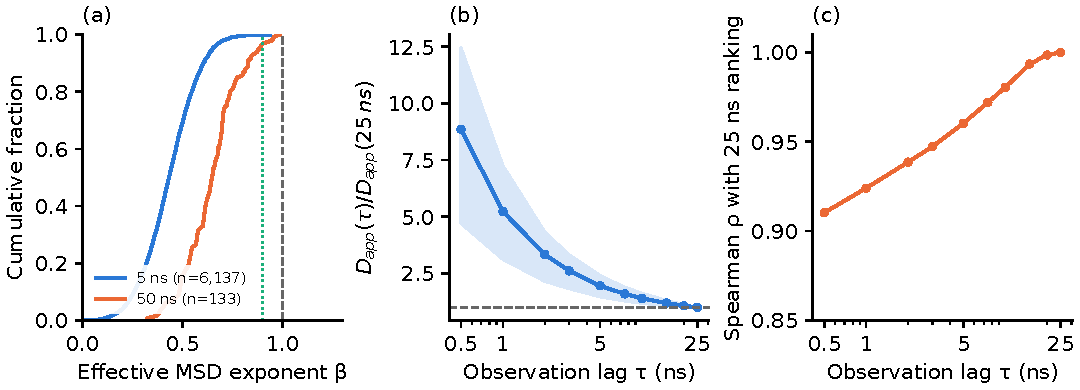
\includegraphics[width=\textwidth]{figures/fig1_time_dependence.pdf}
\caption{Lag dependence of lithium mobility. Left: effective MSD exponents in short and long
runs, with the operational threshold 0.9 and diffusive exponent 1 marked separately.
Middle: $\Dapp(\tau)/\Dapp(25\,\mathrm{ns})$ in the long runs (median and 10th--90th percentiles).
Right: ranking correlation with the 25 ns reference. Lag comparisons share trajectory data.}
\label{fig:regime}\label{fig:long}
\end{figure}

\begin{figure}[ht]
\centering
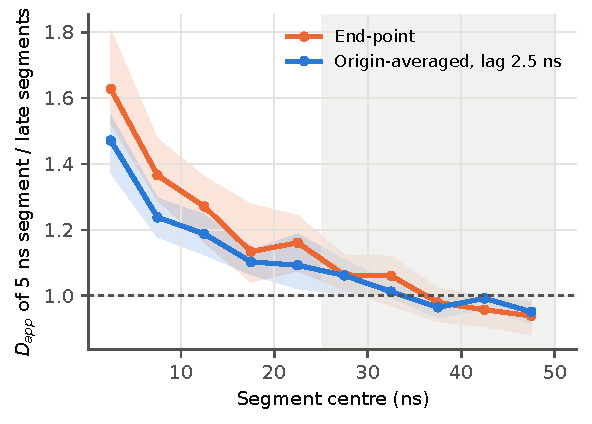
\includegraphics[width=0.6\textwidth]{figures/fig7_segments.pdf}
\caption{Apparent diffusivity of consecutive \SI{5}{\nano\second} segments of the \segN{} long
runs, each computed from its own data, relative to the segments between 25 and
\SI{50}{\nano\second} (shaded): median over systems and 95\% bootstrap interval.}
\label{fig:segments}
\end{figure}

\subsection{Run-to-run noise and its sources}\label{sec:res-noise}
A single \SI{5}{\nano\second} run deviates from the value of its system by a typical factor of
\RepEndFactor{} for the end-point label ($\sigma_{\mathrm{run}}=\RepEndSd$ in log units) and
\RepAvgFactor{} for the origin-averaged one, estimated from pairs of runs of the same system from
different structures (\cref{si:tab:replicas}). Against the spread of the
original screening population, the reliability of one end-point label is \RepEndIcc{} (95\% interval
\RepEndIccLo{} to \RepEndIccHi), and \RepAvgIcc{} (\RepAvgIccLo{} to \RepAvgIccHi) for the origin-averaged
label; the intraclass correlation within the replicated subset agrees (\RepEndIccSub{} and
\RepAvgIccSub). Roughly half of the variance between screened candidates is therefore noise.

The noise has two comparable sources. The \SI{5}{\nano\second} run of each pair agrees with the
first \SI{5}{\nano\second} of its long run, which starts from the same structure, to a median
ratio of \techoEndShortPrefRatio{} with a noise of \techoEndSdDyn, against \RepEndSd{} between
replicas from different structures: the initial structure accounts for
\techoEndFracStructPct\% (\techoEndFracStructLo{} to \techoEndFracStructHi\%) of the run-to-run variance
and the dynamics for the rest; on the \techoEndJointN{} systems with both comparisons, resampled
jointly, the share is \techoEndJointFracStructPct\% (\techoEndJointFracStructLo{} to
\techoEndJointFracStructHi\%). A new pilot of \pilRuns{} runs in \pilN{} systems gives a compatible
same-structure dispersion (\pilSdDyn{} in log units; \cref{si:sec:pilot}). This protocol check
does not validate adaptive allocation or resolve the structural share. The originals, the replicas and the long runs were produced in
different batches of the data set, but none is shifted or differently spread
(Supplementary Material, after \cref{si:tab:replicas}). Re-sampling the structure and averaging the dynamics both reduce the
noise. A replicate that starts from a new structure samples both sources, as ensembles of
independent runs do in other MD applications~\cite{Coveney2016Ensembles}, but it also costs a new
equilibration; this is the classical choice between independent replications and one longer
run~\cite{Alexopoulos1998Output}. Under this decomposition, removing dynamic noise while keeping structural memory unchanged
would give a reliability of \techoEndOneStructMax{}, compared with \techoEndRelTwo{} for the mean
of two independent structures. This is a conditional calculation, not an upper bound for
arbitrarily long MD: these data cannot establish how quickly structural memory fades, and
extension changes the observation window as well as its precision. The noise
also depends on mobility: it is \techoEndSdSlow{} in the slower half of the replicated systems and
\techoEndSdFast{} in the faster half (rank correlation between the absolute difference and the
level $\techoEndHetRho$, $p=\techoEndHetP$), whereas the learning model of the original study assumes
noise independent of the polymer~\cite{Xie2022Accelerating}. Two candidates measured once each
differ by a factor of \RepEndPairFactor{} from noise alone at one standard deviation and up to
\RepEndPairFactorNinetyFive{} at the 95\% level.

Ion aggregation provides limited chemical context. Systems with more lithium in large clusters
are slower and their short labels are more overestimated, but associations with bias and ranking
error weaken after controlling for long-run mobility and their intervals include zero
(Supplementary Material). These exploratory associations do not identify a rearrangement
mechanism. Neither aggregation descriptor has a clear association with replica noise; with two runs per
system this does not rule out chemical differences in noise.

\begin{figure}[ht]
\centering
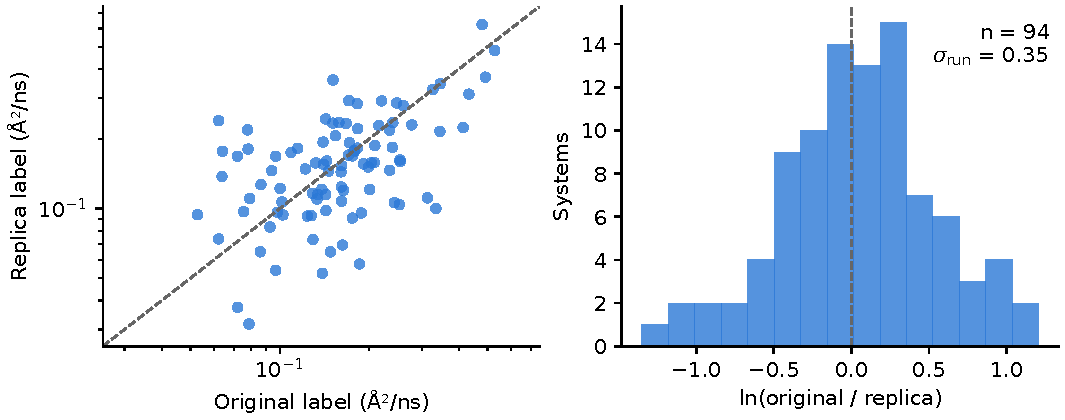
\includegraphics[width=\textwidth]{figures/fig_noise_replicas.pdf}
\caption{Direct evidence of end-point label variability in the \nRep{} replicated screening
systems. Left: original versus independent-initialization label (log axes; dashed identity).
Right: differences of natural-log labels; the noise estimate is their standard deviation divided
by $\sqrt 2$. Differences include both structural and dynamic variation.}
\label{fig:noise}
\end{figure}

\subsection{A noise ceiling for learned predictors}\label{sec:res-ceiling}
Under the additive measurement model, the reliability implies a population correlation ceiling
of \techoEndCorr{} (95\% interval \techoEndCorrLo{} to \techoEndCorrHi) against an independent
end-point label, and an explained-variance ceiling of \techoEndRTwo{} (\cref{tab:ceiling}).
For the origin-averaged label these are \techoAvgCorr{} and \techoAvgRTwo. A finite-sample
correlation can exceed the estimated ceiling. The selection recalls in the table additionally
assume Gaussian system values and noise. Averaging independent initializations raises reliability:
two end-point runs give \techoEndRelTwo{}, four give \techoEndRelFour{}, and reaching 0.8 requires
\techoEndRepForEight{} runs (\techoAvgRepForEight{} for the origin-averaged label).

A fingerprint random forest gives out-of-fold Pearson correlation \mlCorr{} (95\% interval
\mlCorrLo{} to \mlCorrHi; $R^2=\mlRTwo$) on the same screening population (\cref{tab:ml}).
This is compatible with the estimated ceiling, but the wide ceiling interval prevents a claim
that model performance has saturated. Chemical-family splits give \mlFamFineCorr{} and
\mlFamCoarseCorr{}; their nearest training neighbours still have appreciable similarity
(Supplementary Material), so they test interpolation within this chemical space.

In replicated systems, correlation rises from \mlRepA{} and \mlRepB{} against the single labels
to \mlRepMean{} against their mean, consistent with the measurement-model prediction
\mlRepMeanExp{} (gain 95\% interval \mlRepGainLo{} to \mlRepGainHi). Replicated evaluation labels
therefore help distinguish model error from evaluation noise. They do not make better models
unnecessary. Xie et al. already demonstrated denoising and estimated performance equivalent to
about four simulations for conductivity~\cite{Xie2022Accelerating}; our analysis expresses the
label uncertainty relative to the population and its consequences for metrics.

Against long-run screening references, the model and a system's own short run have rank
correlations \mlLongScreenModel{} and \mlLongScreenShort{}. For literature polymers evaluated
externally, these are \mlLongLitModel{} and \mlLongLitShort{}. Shared initial structures favour
the short-run comparison, and neither reference establishes equilibrium transport.
System-level splits remain necessary; the trajectory-split check is reported in the Supplementary
Material.

\begin{table}[ht]
\centering
\caption{Noise ceiling of short-run labels in the screening population: reliability of the mean of
$n$ runs, model-implied population correlation ceiling, and Gaussian-model recall of the highest expected short-run labels. Origin-averaged labels use lag $T/2$.}\label{tab:ceiling}
{\footnotesize% Generado por techo.py. No editar a mano.
\begin{tabular}{lrrrrrr}
\toprule
 & & & & \multicolumn{3}{c}{Recall of the true top} \\
\cmidrule(lr){5-7}
Label & Runs & Reliability & Ceiling & 5\% & 10\% & 20\% \\
\midrule
End-point & 1 & 0.44 & 0.66 & 36\% & 43\% & 54\% \\
 & 2 & 0.61 & 0.78 & 46\% & 54\% & 63\% \\
 & 3 & 0.70 & 0.84 & 54\% & 61\% & 68\% \\
 & 4 & 0.76 & 0.87 & 58\% & 65\% & 72\% \\
\addlinespace
Origin-averaged & 1 & 0.54 & 0.74 & 43\% & 50\% & 59\% \\
 & 2 & 0.70 & 0.84 & 53\% & 61\% & 68\% \\
 & 3 & 0.78 & 0.88 & 61\% & 67\% & 73\% \\
 & 4 & 0.83 & 0.91 & 65\% & 70\% & 76\% \\
\bottomrule
\end{tabular}
}
\end{table}

\begin{table}[ht]
\centering
\caption{Out-of-sample correlation of a random forest on monomer fingerprints with short-run
labels (cross-validation split by system, or by chemical family of the monomer), against the
noise ceiling of each label. The ceilings and their intervals rest on the run-to-run noise of
the \nRep{} replicated systems, not on the \mlNSys{} systems of the first rows.}\label{tab:ml}
{\small\setlength{\tabcolsep}{3pt}% Generado por ml_demo.py. No editar a mano.
\begin{tabular}{p{0.33\textwidth}rrr}
\toprule
Evaluation target & Systems & Pearson $r$ (95\% CI) & Ceiling (95\% CI) \\
\midrule
One label, system split & 6{,}003 & 0.69 (0.68 to 0.71) & 0.66 (0.52 to 0.78) \\
Fine families (Tanimoto $\geq$ 0.6) & 6{,}003 & 0.69 (0.67 to 0.70) & 0.66 (0.52 to 0.78) \\
Coarse families (Tanimoto $\geq$ 0.4) & 6{,}003 & 0.69 (0.68 to 0.70) & 0.66 (0.52 to 0.78) \\
Replicas, first / second & 94 & 0.64 / 0.68 & 0.66 (0.52 to 0.78) \\
Mean of two replicas & 94 & 0.76 (0.63 to 0.84) & 0.78 (0.65 to 0.87) \\
\bottomrule
\end{tabular}
}
\end{table}

\subsection{Selecting candidates from one short run}\label{sec:res-selection}
For the \nPairs{} systems simulated at both lengths, the end-point label of the
\SI{5}{\nano\second} run is a median \PairEndRatio{} times the long-run reference (10th to 90th percentile range
\PairEndLo{} to \PairEndHi; \cref{si:fig:pairs}), and the Spearman correlation between them is
\PairEndRho{} (95\% interval \PairEndRhoLo{} to \PairEndRhoHi). The correlation owes much to the wide
range of mobilities in this subset: it is \PairEndRhoLit{} among the \nLongLit{} literature
polymers but \PairEndRhoScreen{} among the \nLongScreen{} screening polymers. In the whole
paired set the short run identifies \PairEndTopTenHits{} of the \PairEndTopTenK{} best systems
(\cref{tab:selection}), but these top sets consist almost entirely of literature polymers
(\LitInTopTen{} of \PairEndTopTenK{} and \LitInTopTwenty{} of \PairEndTopTwentyK), which are easy to
separate. Within the \ScrN{} screening polymers the short run still recovers \ScrTopTenHits{} of
the \ScrTopTenK{} best and \ScrTopTwentyHits{} of the \ScrTopTwentyK{} best, against 10\% and 20\%
by chance. These recalls are optimistic, because the short and long runs of a pair share their
initial structure. A short run therefore provides useful coarse screening while uncertain
differences limit fine ranking.

The median ratio of \PairEndRatio{} is larger than the \ratioFive{} obtained at the same lag from
the origin-averaged long curves, and this slowdown explains the gap. The short runs behave like the
first \SI{5}{\nano\second} of the long runs (median ratio \techoEndShortPrefRatio), and that
first segment is \segEndFirstVsAll{} times faster than the average of all segments, which is
roughly what separates a single early window from a curve averaged over all time origins. Short
labels in the dataset are therefore systematically biased upwards by the early, faster part of
the trajectory, and more so for the screening polymers. For ranking, this bias matters only to the
extent that it differs between systems.

\begin{table}[ht]
\centering
\caption{Recall of the best systems according to the \SI{50}{\nano\second} reference when they are
selected from the \SI{5}{\nano\second} run of the same system (\nPairs{} systems; the last rows
only the \ScrN{} screening polymers). Intervals by bootstrap over systems; ``Random'' is the expected
recall of a random selection of $k$ systems. All recalls are optimistic, because the two runs of a
pair share their initial structure.}
\label{tab:selection}
% Generado por incertidumbre.py. No editar a mano.
\begin{tabular}{lrrrrr}
\toprule
Estimator, \SI{5}{\nano\second} run & Top & $k$ & Hits & Recall (95\% CI) & Random \\
\midrule
End-point & 5\% & 7 & 7 & 100\% (50 to 100) & 5\% \\
 & 10\% & 13 & 11 & 85\% (62 to 100) & 10\% \\
 & 20\% & 27 & 23 & 85\% (71 to 94) & 20\% \\
Origin-averaged, lag $T/2$ & 5\% & 7 & 6 & 86\% (50 to 100) & 5\% \\
 & 10\% & 13 & 10 & 77\% (62 to 100) & 10\% \\
 & 20\% & 27 & 22 & 81\% (75 to 94) & 20\% \\
End-point, screening only & 5\% & 5 & 4 & 80\% (67 to 100) & 5\% \\
 & 10\% & 10 & 7 & 70\% (50 to 86) & 10\% \\
 & 20\% & 19 & 14 & 74\% (54 to 83) & 20\% \\
\bottomrule
\end{tabular}

\end{table}

\subsection{Estimators and stopping within a run}\label{sec:res-stopping}
Prefix estimates overstate the finite-lag reference: at \SI{5}{\nano\second}, typical errors are
$\times\preEndErrFive$ for the end-point and $\times\preFitErrFive$ for a linear fit.
Power-law extrapolation reduces error against $\Dapp(25\,\mathrm{ns})$ to
$\times\prePowErrFive$, but underestimates the late MSD slope (median ratio
\refPowSlopeRatioFive; \cref{si:tab:sens-prefix-ref}). A subdiffusive power law does not approach
normal diffusion; this is an empirical estimate of a specified finite-lag quantity.

For the rules and reference tested, exponent- and precision-based stopping do not improve the
fixed-length cost--error frontier (\cref{si:fig:prefix,si:fig:frontier,si:tab:rules}). Settings
selected on half the systems can miss their target on the held-out half
(\cref{si:tab:frontier}). The shared reference data and conditional ion bootstrap limit this
comparison. It does not rule out other stopping rules or establish that replication is preferable
to extension for estimating equilibrium transport.



\subsection{Spending the budget across candidates: adaptive allocation}\label{sec:res-allocation}
The noise model measured above is compatible with the replicated systems: the
differences between replicas show no departure from a Gaussian (excess kurtosis \alKurt,
Shapiro-Wilk $p=\alShapiroP$).
With it, how replicates are distributed matters more than how many are run (\cref{fig:allocation};
values in \cref{si:tab:allocation}). Uniform replicates improve slowly: for the top 10\% of \alN{} candidates
the recall rises from \alUnifTopTenBOne\% with one run to \alUnifTopTenBFour\% with four.
Boundary-focused allocation reaches \alBoundTopTenBTwo\% with two runs per candidate on average
and \alBoundTopTenBFour\% with four, and matches four uniform replicates with
\alEqTopTenUnifFour{} runs per candidate, a saving of $\times$\alSavingTopTenUnifFour. The saving
grows with the selectivity of the target: $\times$\alSavingTopFiveUnifFour{} for the top 5\% and
$\times$\alSavingTopOneUnifFour{} for the top 1\% (\cref{si:tab:alloc-eq}). Successive halving, which re-runs the current leaders in repeated rounds, performs
similarly: with the end-point label it is better for the top 1\% at small budgets
(\alHalvingTopOneBOneQuarterEnd\% against \alBoundTopOneBOneQuarterEnd\% with 1.25 runs per
candidate), and with the origin-averaged label it is worse at larger budgets
(\alHalvingTopOneBFourAvg\% against \alBoundTopOneBFourAvg\% with four).
Even a two-stage re-screening, in which the budget left after the first run is spread evenly over
a fixed shortlist of the best candidates, captures most of the gain: with a shortlist of the best $4k$ fixed in advance it saves
$\times$\alTwoStageFourkSavingTopOne{} for the top 1\%, $\times$\alTwoStageFourkSavingTopFive{}
for the top 5\% and $\times$\alTwoStageFourkSavingTopTen{} for the top 10\%, and the best of three
shortlist sizes in hindsight gives ($\times$\alTwoStageSavingTopOne,
$\times$\alTwoStageSavingTopFive{} and $\times$\alTwoStageSavingTopTen). Most of the saving therefore comes from not
spending replicates on candidates that the first run already places far from the cut-off;
allocating them where the selection is still in doubt adds the rest, and does so without a
shortlist size to tune. The price is sequential work: in batches of \alBatchPct\% of the
candidates, matching four uniform replicates takes \alRoundsTopTen{} additional rounds of simulation and
analysis for the top 10\% and \alRoundsTopOne{} for the top 1\%, against a single extra round
for the two-stage re-screening. Where each round waits in a queue, the two-stage scheme is the
practical alternative, but its saving depends on the shortlist size and should be evaluated
with that choice fixed in advance. Nor does the saving depend on knowing the
reliability exactly: planning with $r=\alRelPlanLo$ or $\alRelPlanHi$ instead of \alRelTrue{} gives
savings of $\times$\alMisLoSavingTopTen{} and $\times$\alMisHiSavingTopTen{} for the top 10\%
(\cref{si:tab:alloc-checks}), and if the true reliability lies at either end of its interval the
saving is $\times$\alTrueLoSavingTopTen{} to $\times$\alTrueHiSavingTopTen{} for the top 10\% and
$\times$\alTrueLoSavingTopOne{} to $\times$\alTrueHiSavingTopOne{} for the top 1\%. The result holds with the empirical distribution of the
short runs and with the origin-averaged label, and knowing that slow systems are noisier does not
improve the allocation (Supplementary Material). For the expected short-run target and this noise model, an initial run followed by selective
new-structure replication is preferable to uniform replication at the tested budgets.

These gains are predictions of the noise model, since the public data contain at most two runs per
system; the replicated systems allow only a partial check, which is consistent with them but has
little statistical power (\cref{si:tab:val-alloc}). The
model's probabilities of exceeding the top-10\% cut-off are informative on real runs, improving the
Brier score of the base rate by \valAlBrierGainTen\% with a calibration slope of
\valAlCalSlopeTen{} (95\% interval \valAlCalSlopeLoTen{} to \valAlCalSlopeHiTen). In the real
campaign on \valAlNCamp{} systems, sending the \valAlExtra{} second runs to the boundary recovers
\valAlBoundTen\% of the top 10\% according to the long runs, as many as giving a second run to
every system (\valAlBothTen\%), against \valAlRandomTen\% for randomly placed second runs and
\valAlOnlyATen\% with first runs only. With \valAlKTen{} systems in the top set the difference from
random placement is not significant (95\% interval from $\valAlDiffLoTen$ to
$+\valAlDiffHiTen$ percentage points), and for the top 20\% no strategy improves on the first run
alone. The long runs share their structure with the first runs, which probably favours the first
run over any second run from a new structure, by an amount we cannot quantify. The calibration
check, in turn, concerns a second noisy run rather than the latent value that the allocation
targets. Noise parameters for the campaign are fitted to the available campaign pairs. The real
runs therefore do not contradict the simulated gains, but they cannot show that
adaptive allocation beats random placement.

\begin{figure}[ht]
\centering
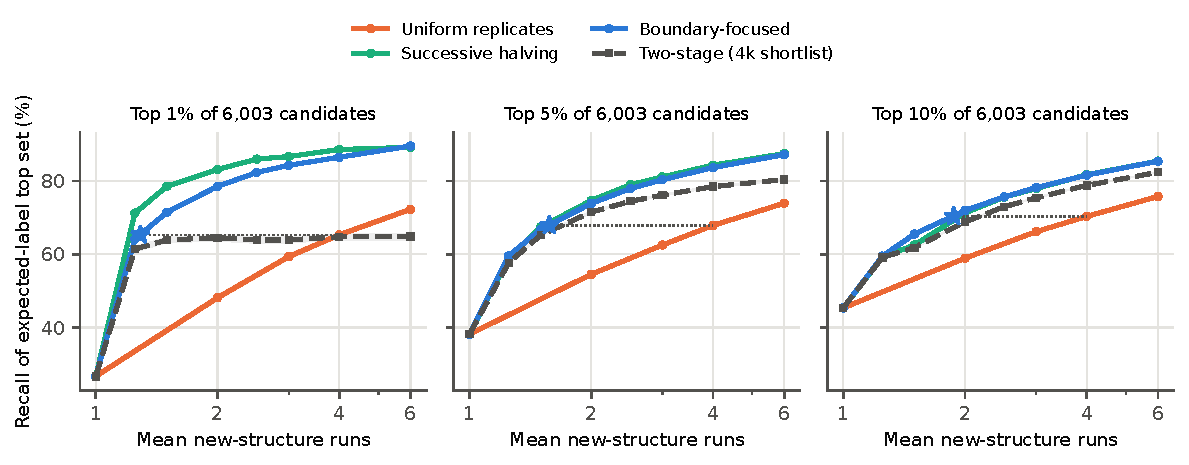
\includegraphics[width=\textwidth]{figures/fig8_allocation.pdf}
\caption{Recall of the true top set as a function of the mean number of \SI{5}{\nano\second} runs
per candidate, for four ways of allocating the budget (\alReps{} simulated campaigns of \alN{}
candidates with the measured noise; each run starts from a new, equilibrated structure). The
true top set is the top $k$ by the expected \SI{5}{\nano\second} label of each system, not by its
long-time diffusivity. The two-stage shortlist is fixed at $4k$. Bands show 95\% Monte Carlo
intervals conditional on the calibrated model; markers show boundary budgets matching four
uniform replicates.}\label{fig:allocation}
\end{figure}


\subsection{Related transport labels}\label{sec:res-general}
\ifconductivityready
The anion diffusivity and the platform's cluster Nernst--Einstein conductivity
extend the audit to related observables (\cref{tab:general}). The latter combines end-point ion
diffusivities and cluster populations~\cite{FranceLanord2019NernstEinstein}; we use the distributed
labels in their reported units. This analysis does not establish the accuracy of those absolute
units or validate the cluster approximation against collective charge displacement.
For a matched ion comparison we use origin-averaged diffusivities at half the run length.

Anion labels are more reliable than lithium labels (\genTfsiRel{} against \genLiRel), and their
short--long ranking agreement is higher (\genTfsiRhoScreen{} against \genLiRhoScreen{} among
screening systems). Correlations against replica means increase for both ions. The conductivity
has reliability \genCondRel{} (95\% interval \genCondRelLo{} to \genCondRelHi), with predictor
correlation \genCondMl{} and estimated ceiling \genCondCeil. These point comparisons do not
identify which chemical information the predictor lacks. Calibrated constant-noise campaigns
again predict savings from adaptive replication, conditional on their expected-label targets.

Choosing the physical label matters. In screening runs, lithium diffusivity and conductivity have
rank correlation \genCondVsLiRhoShort{} and their top deciles overlap by
\genCondVsLiTopTenPct\%, despite correlated replica differences (\genCondVsLiNoiseCorr).
A conductivity screening campaign therefore needs a conductivity target. Agreement across these
observables supports the audit within HTP-MD, but they share trajectories and physical information
and are not independent tests of transfer to other regimes.

\else
The origin-averaged TFSI diffusivity at half the run length provides a related observable on the
same screening population (\cref{tab:general}). Its reliability is \genTfsiRel{} against
\genLiRel{} for lithium, with estimated population ceilings \genTfsiCeil{} and \genLiCeil{}.
The fingerprint model gives correlations \genTfsiMl{} and \genLiMl{} against single labels.
Against the mean of two replicas, the anion correlation rises to \genTfsiMlMean{}, compared
with the measurement-model expectation \genTfsiMlMeanExp{}. The screening short--long rank
correlation is \genTfsiRhoScreen{} for TFSI and \genLiRhoScreen{} for lithium.

Constant-noise campaign simulations predict savings of $\times$\genTfsiSaving{} and
$\times$\genLiSaving{} for the top decile by expected short-run label. These related observables
share trajectories and are not independent tests of transfer across simulation regimes.
The conductivity analysis is excluded from this working revision until the original per-run
conductivity input can be recovered and recalculated on the same population.
\fi

\begin{table}[ht]
\centering
\caption{Results for the origin-averaged ion diffusivities at half the run length
\ifconductivityready and the platform's cluster conductivity\fi.
The population is one original label per screening system; noise comes from \nRep{} replica pairs.
Allocation uses constant noise and targets expected short-run labels.}\label{tab:general}
\resizebox{\textwidth}{!}{% Generado por generalidad.py. No editar a mano.
\begin{tabular}{lrr}
\toprule
 & \Li{} & TFSI$^-$ \\
\midrule
Run-to-run noise (log) & 0.28 & 0.19 \\
Noise, slow / fast half & 0.29 / 0.26 & 0.20 / 0.18 \\
Reliability (95\% CI) & 0.54 (0.40 to 0.67) & 0.79 (0.74 to 0.84) \\
Noise ceiling & 0.74 & 0.89 \\
Random forest vs one label & 0.76 & 0.85 \\
Random forest vs two-run mean (expected) & 0.82 (0.84) & 0.89 (0.90) \\
Spearman with 50 ns run, screening & 0.70 & 0.83 \\
Spearman with 50 ns run, literature & 0.94 & 0.96 \\
Runs matching 4 uniform replicates (top 10\%) & 1.8 ($\times$2.3) & 1.5 ($\times$2.7) \\
\bottomrule
\end{tabular}
}
\end{table}

\subsection{Practical guidance}\label{sec:res-guide}
The recommendations in \cref{tab:guide} apply to the studied protocol, not to universal MD lengths.
Before production, check energy drift and relevant structural and dynamical observables;
stationary energy alone does not establish transport convergence. Report the estimator, lag and
MSD regime. Prefer origin-averaged labels and distinguish within-run precision from accuracy
against a long-time coefficient. Choose the physical target explicitly: lithium self-mobility
and conductivity rank different candidates because correlated ion motion can carry little net
charge~\cite{FranceLanord2019NernstEinstein}.

\begin{table}[ht]
\centering
\caption{Decisions supported by this case study.}
\label{tab:guide}
\small\setlength{\tabcolsep}{4pt}
\begin{tabular}{@{}>{\raggedright\arraybackslash}p{0.22\textwidth}>{\raggedright\arraybackslash}p{0.34\textwidth}>{\raggedright\arraybackslash}p{0.36\textwidth}@{}}
\toprule
Objective & Action & Main limitation \\
\midrule
Coarse screening & One short run; use an origin-averaged label & Similar candidates remain hard to separate \\
\addlinespace
Select by expected short-run label & Replicate uncertain candidates; use a fixed shortlist if sequential rounds are costly & Savings are calibrated-model predictions, not validated savings for equilibrium transport \\
\addlinespace
Compare similar candidates & Use independent initial structures & Replication reduces variance, not necessarily temporal bias \\
\addlinespace
Evaluate a learned model & Split by system; use replicated test labels & The estimated population ceiling is uncertain and model-dependent \\
\addlinespace
Estimate equilibrium transport & Extend and test relaxation and lag stability & Even \SI{50}{\nano\second} rarely establishes the diffusive regime here \\
\bottomrule
\end{tabular}
\end{table}



\subsection{Limitations}\label{sec:limitations}
All systems share one force field, one temperature and one salt; the examined transport labels
are related observables and the numbers are
specific to this setting, and the workflow, not the values, is what transfers to other campaigns.
The long runs of the literature polymers were chosen by the dataset's authors; the screening
systems with a replica (\nRep) or a long run (\nLongScreen) show no detected difference in their marginal labels from the rest of the
screening set, but they are few and largely the same systems (\techoEndReprOverlap{} in common). The reference lag of \SI{25}{\nano\second} is not a
converged limit and shares data with the truncated trajectories, so prefix-based errors at long
$T$ are optimistic. Self-diffusion is only a proxy for conductivity, and the cluster Nernst-Einstein conductivity
neglects correlations between different clusters~\cite{FranceLanord2019NernstEinstein}; finite-size
effects~\cite{Yeh2004SystemSize} are not corrected. The boxes are small (\tamBoxMin{} to
\SI{\tamBoxMax}{\nano\metre} side, \tamChainsMin{} to \tamChainsMax{} chains), so each
initial structure samples few chain conformations and packings; the structural part of the noise
may be smaller in larger boxes, which would raise the reliability of a single run. The structural attribution additionally assumes
independent dynamical histories; shared equilibration and system-specific batch effects cannot
be excluded. We do not establish that the structural contribution persists at arbitrary run lengths. The noise model rests on \nRep{} replicated
pairs: the allocation gains are predictions of a model that the real runs, with \valAlNCamp{} systems,
do not contradict but cannot confirm; a campaign with several replicates per candidate would test
them directly. No allocation result establishes the best policy for long-time transport when
short-run biases change the ranking. The observables share trajectories and physical
information, so their agreement is not independent cross-domain validation. The small SCAYLE
pilot checks protocol consistency; its annealed structures follow a different preparation and
it cannot validate the allocation gains (\cref{si:sec:pilot}). The analysis is largely exploratory: windows, thresholds, estimators and strategies
were compared on the same data, and only the stopping-rule settings were chosen and evaluated on
separate halves of the systems.

% =============================================================================
\section{Conclusions}\label{sec:conclusion}
This audit separates two limitations of short MD labels: their mobility depends on observation
lag and decreases with trajectory age, while independent initializations give substantial
run-to-run variation. Replica noise accounts for about half the screening-label variance.
The inferred prediction ceiling is uncertain; a fingerprint model is compatible with it, but
model saturation is not established. The structural attribution is conditional on the assumed
noise decomposition and does not prove irreducibility under longer simulation.

Calibrated campaign simulations predict substantial savings from selective replication when the
objective is the expected short-run label. A single re-screening round retains much of the gain;
the available real runs cannot confirm superiority over random placement. These savings do not
establish recovery of the best equilibrium transport properties. The related transport-label analyses support the usefulness of the audit within this dataset, while their
numerical reliabilities differ. The transferable contribution is a procedure for specifying the
label, measuring its noise and time dependence, and evaluating decisions against the intended
physical target.



\section*{Data and code availability}
The HTP-MD trajectories and curves are publicly available from the Toyota Research Institute
platform~\cite{Xie2023HTPMD}. The analysis scripts, the per-trajectory result tables and the
scripts that generate every number, table and figure of this paper are available at
\url{https://github.com/fhernandogallego/md-label-reliability} with the original analysis snapshot archived on Zenodo
(\url{https://doi.org/10.5281/zenodo.23483460}); the revised scripts and derived inputs accompany
this revision, and the raw trajectories are not redistributed. The
analysis scripts were written with the assistance of Claude (Anthropic) and revised with Codex (OpenAI); the authors reviewed
and verified the code. The scripts regenerate tables and figures from the released derived inputs.
The SCAYLE pilot intervals are archived summary results; their per-run inputs are not included
in the compact-input workflow, so those bootstrap intervals are not independently recomputed there.

\section*{Supplementary material}
Supplementary Material associated with this article (data set details and validation of the
trajectory processing; sensitivity of the regime census and of the lag dependence; run-to-run
reproducibility; end-point estimator; paired runs; prefix-based estimators, stopping rules and
held-out evaluation; within-run slowdown; exploratory ion aggregation; the new SCAYLE protocol pilot; robustness of the adaptive allocation and its check on
real runs) is provided as a separate file.

\section*{CRediT authorship contribution statement}
\par\noindent\textbf{Francisco Hernando-Gallego:}\par\noindent Conceptualization, Methodology, Software, Formal analysis,
Writing (original draft), Supervision.
\par\noindent\textbf{Dimitar Vasilev-Vasilev:}\par\noindent Software, Data curation, Investigation, Validation, Writing
(review \& editing).
\par\noindent\textbf{Diego Garc\'ia-Santos:}\par\noindent Investigation, Validation, Writing (review \& editing).
\par\noindent\textbf{Alfonso Campo-Camacho:}\par\noindent Validation, Writing (review \& editing).
\par\noindent\textbf{Alberto G\'omez-G\'omez:}\par\noindent Validation, Writing (review \& editing).

\section*{Declaration of competing interest}
The authors declare that they have no known competing financial interests or personal
relationships that could have appeared to influence the work reported in this paper.

\section*{Funding}
This research did not receive any specific grant from funding agencies in the public, commercial,
or not-for-profit sectors.

\section*{Acknowledgements}
The authors acknowledge SCAYLE (Supercomputaci\'on Castilla y Le\'on, Le\'on, Spain) for
providing access to its computing infrastructure.

\section*{Declaration of generative AI and AI-assisted technologies in the manuscript preparation process}
During the preparation of this work the authors used Claude (Anthropic) and Codex (OpenAI) to assist with
writing and editing the manuscript, as none of the authors is a native English speaker. After
using this tool, the authors reviewed and edited the content as needed and take full
responsibility for the content of the publication.

\bibliographystyle{elsarticle-num}
\bibliography{references}

\end{document}
